%\listfiles
\documentclass[diss]{mdtufsm}
% um tipo específico de monografia pode ser informado como parâmetro opcional:
%\documentclass[tese]{mdtufsm}
% a opção `openright' pode ser usada para forçar inícios de capítulos
% em páginas ímpares
% \documentclass[openright]{mdtufsm}
% para gerar uma versão frente-e-verso, use a opção 'twoside':
% \documentclass[twoside]{mdtufsm}

\usepackage[T1]{fontenc}        % pacote para conj. de caracteres correto
\usepackage{fix-cm} %para funcionar corretamente o tamanho das fontes da capa
\usepackage{times, color, xcolor}       % pacote para usar fonte Adobe Times e cores
\usepackage[utf8]{inputenc}   % pacote para acentuação
\usepackage{graphicx}  % pacote para importar figuras
\usepackage{amsmath,latexsym,amssymb} %Pacotes matemáticos
\usepackage{listings}
\usepackage{url}
\usepackage[%hidelinks%, 
            bookmarksopen=true,linktoc=none,colorlinks=true,
            linkcolor=black,citecolor=black,filecolor=magenta,urlcolor=blue,
            pdftitle={Desenvolvimento de um escalonador sensível ao contexto para o Apache Hadoop},
            pdfauthor={Guilherme Weigert Cassales},
            pdfsubject={Trabalho de Graduação},
            pdfkeywords={Apache Hadoop, escalonador, sensível ao contexto, Informática, UFSM}
            ]{hyperref} %hidelinks disponível no pacote hyperref a partir da versão 2011-02-05  6.82a
%Nesse caso, hidelinks retira os retângulos em volta dos links das referências

%Margens conforme MDT 7ª edição, arrumar diretamente no mdtufsm.cls para funcionar a opção twoside *PENDENTE*
\usepackage[inner=30mm,outer=20mm,top=30mm,bottom=20mm]{geometry} 
\usepackage{epstopdf}
\usepackage{graphicx}


%==============================================================================
% Se o pacote hyperref foi carregado a linha abaixo corrige um bug na hora
% de montar o sumário da lista de figuras e tabelas
% Se o pacote não foi carregado, comentar a linha %
%==============================================================================

%%=============================================================================
%% Trampa para corrigir o bug do hyperref que redefine o caption das figuras e das
%% tabelas, n�o colocando o nome ``Figura'' antes do n�mero do mesmo na lista
%%=============================================================================

\makeatletter

\long\def\@caption#1[#2]#3{%
  \expandafter\ifx\csname if@capstart\expandafter\endcsname
                  \csname iftrue\endcsname
    \global\let\@currentHref\hc@currentHref
  \else
    \hyper@makecurrent{\@captype}%
  \fi
  \@ifundefined{NR@gettitle}{%
    \def\@currentlabelname{#2}%
  }{%
    \NR@gettitle{#2}%
  }%
  \par\addcontentsline{\csname ext@#1\endcsname}{#1}{%
    \protect\numberline{\csname fnum@#1\endcsname ~-- }{\ignorespaces #2}%
  }%
  \begingroup
    \@parboxrestore
    \if@minipage
      \@setminipage
    \fi
    \normalsize
    \expandafter\ifx\csname if@capstart\expandafter\endcsname
                    \csname iftrue\endcsname
      \global\@capstartfalse
      \@makecaption{\csname fnum@#1\endcsname}{\ignorespaces#3}%
    \else
      \@makecaption{\csname fnum@#1\endcsname}{%
        \ignorespaces
        \ifHy@nesting
          \expandafter\hyper@@anchor\expandafter{\@currentHref}{#3}%
        \else
          \Hy@raisedlink{%
            \expandafter\hyper@@anchor\expandafter{%
              \@currentHref
            }{\relax}%
          }%
          #3%
        \fi
      }%
    \fi
    \par
  \endgroup
}

\makeatother

%==============================================================================
% Identificação do trabalho
%==============================================================================
\title{Escalonamento Adaptativo para o Apache Hadoop}

\author{Cassales}{Guilherme Weigert}

\course{Curso de Ciência da Computação}
\altcourse{Curso de Ciência da Computação}

\institute{Centro de Tecnologia}
\degree{Mestre em Ciência da Computação}

% Número do TG (verificar na secretaria do curso)
% Para mestrado deixar sem opção dentro do {}
\trabalhoNumero{}

%Orientador
\advisor[]{Profª. Drª.}{Charão}{Andrea Schwertner}
%Se for uma ``orientadora'' descomentar a linha baixo
\orientadoratrue

%Avaliadores (Banca)
\committee[Prof. Dr.]{Stein}{Benhur de Oliveira}{UFSM}
\committee[Profª. Drª.]{Barcelos}{Patrícia Pitthan de Araújo}{UFSM}


% a data deve ser a da defesa; se nao especificada, são gerados
% mes e ano correntes
\date{20}{Janeiro}{2016}

%Palavras chave
\keyword{Apache Hadoop} 
\keyword{Escalonador}
\keyword{Sensibilidade ao Contexto}

%%=============================================================================
%% Início do documento
%%=============================================================================
\begin{document}

%%=============================================================================
%% Capa e folha de rosto
%%=============================================================================
\maketitle

%%=============================================================================
%% Catalogação (obrigatório para mestrado) e Folha de aprovação
%%=============================================================================
%Somente obrigatório para dissertação, para TG, remover as linhas	77	%
%Como a CIP vai ser impressa atrás da página de rosto, as margens inner e outer	
%devem ser invertidas.
\newgeometry{inner=20mm,outer=30mm,top=30mm,bottom=20mm}	
\makeCIP{cassales@inf.ufsm.br} %email do autor		
\restoregeometry

%Se for usar a catalogação gerada pelo gerador do site da biblioteca comentar as linhas
%acima e utilizar o comando abaixo
%\includeCIP{CIP.pdf}

%folha de aprovação
\makeapprove


%%=============================================================================
%% Agradecimentos (opcional)
%%=============================================================================
%\chapter*{Agradecimentos}
%Agradeço à minha família por todo apoio, não só durante os longos anos de graduação, mas em todas as etapas de minha vida.
%
%À minha namorada Raíssa, não só pelo apoio em mais um TG e mais uma graduação, mas por todo crescimento conjunto que tivemos durante um ano e quase noventa meses.
%
%Aos amigos mais próximos, que mesmo estando fisicamente distantes ou que a rotina tenha impedido um convívio diário, por sempre estarem dispostos a compartilhar experiências.
%
%À professora Andrea Charão, por todo suporte prestado tanto no papel de orientadora como de coordenadora do curso.
%
%Agradeço também, a todos que tornaram possível e/ou participaram na realização deste trabalho.


%%=============================================================================
%% Resumo
%%=============================================================================
\begin{abstract}
Hoje em dia, o volume de dados gerados é muito maior do que a capacidade de processamento dos computadores. Como solução para esse problema, algumas tarefas podem ser paralelizadas ou distribuidas. O \emph{framework Apache Hadoop} \cite{Hadoop}, é uma delas e poupa o programador as terefas de gerenciamento, como tolerância à falhas, particionamento dos dados entre outros.
Um problema no escalonador do \emph{Apache Hadoop} é que seu foco é em ambientes homogêneos, o que muitas vezes não é possível de se manter. O foco deste trabalho foi na melhora de um escalonador já existente, possuindo como objetivo torná-lo sensível ao contexto, permitindo que as capacidades físicas de cada máquina sejam consideradas na hora da distribuição das tarefas submetidas. Optou-se por inserir coletores de informações de contexto (memória e cpu) no  CapacityScheduler, tornando o comportamento desse sensível ao contexto. Através das mudanças feitas e de experimentos feitos usando um benchmark bem conhecido (TeraSort), foi possível demonstrar uma melhora no escalonamento em relação ao escalonador original com a configuração padrão.
\end{abstract}


%%=============================================================================
%% Abstract
%%=============================================================================
% resumo em inglês

\begin{englishabstract}
{Development of a context-aware scheduler for Apache Hadoop}
{Undergraduate Program in Computer Science}
{Apache Hadoop. Scheduler. Context-aware}
{January}
{th}
Nowadays the volume of data generated by the services provided for end users, is way larger than the processing capacity of one computer alone. As a solution to this problem, some tasks can be parallelized. The Apache Hadoop framework, is one of these parallelized solutions and it spares the programmer of management tasks such as fault tolerance, data partitioning, among others.
One problem on this framework is the scheduler, which is designed for homogeneous environments. It is worth to remember that maintaining a homogeneous environment is somewhat difficult today, given the fast development of new, cheaper and more powerful hardware. This work focuses on altering the Capacity Scheduler, in order to make it more context-aware towards resources on the cluster. Making it possible to consider the the physical capacities of the machines when scheduling the submitted tasks. It was chosen to insert context information (memory and cpu) collectors on CapacityScheduler, making his scheduling more context-aware. Through the changes and experiments made using a common and well known benchmark (TeraSort), it was possible to notice a improvement on scheduling in relation to the original scheduler using the default configuration.
\end{englishabstract}

%% Lista de Ilustrações (opc)
%% Lista de Símbolos (opc)
%% Lista de Anexos e Apêndices (opc)

%%=============================================================================
%% Lista de figuras (comentar se não houver)
%%=============================================================================
%\renewcommand{\listfigurename}{Figure List}
\listoffigures


%%=============================================================================
%% Lista de tabelas (comentar se não houver)
%%=============================================================================
%%\listoftables

%%=============================================================================
%% Lista de Apêndices (comentar se não houver)
%%=============================================================================
%\renewcommand{\listappendixname}{Appendix List}
\listofappendix

%%=============================================================================
%% Lista de Anexos (comentar se não houver)
%%=============================================================================
%\listofannex

%%=============================================================================
%% Lista de abreviaturas e siglas
%%=============================================================================
 %o parametro deve ser a abreviatura mais longa
%\begin{listofabbrv}{UbiComp}
%   \item [BNF] \textit{Backus-Naur Form}
%   \item [UbiComp] Computação Ubíqua
%\end{listofabbrv}


%%=============================================================================
%% Lista de simbolos (opcional)
%%=============================================================================
%Simbolos devem aparecer conforme a ordem em que aparecem no texto
% o parametro deve ser o símbolo mais longo
%\begin{listofsymbols}{teste}
%  \item [$\varnothing$] vazio
%  \item [$\Gamma$]  Gama
%  \item [$\forall$] Para todo
%\end{listofsymbols}

%%=============================================================================
%% Sumário
%%=============================================================================
%\renewcommand{\contentsname}{Index}
%\renewcommand{\appendixsname}{Appendix}
\tableofcontents

%%=============================================================================
%% Início da dissertação
%%=============================================================================
\setlength{\baselineskip}{1.5\baselineskip}

%Adiciona cada capitulo
\chapter{Introduction}
\label{chap:Introduction}
One of the major IT companies nowadays, known as Google \cite{Google}, had the initial idea of a way to process a huge data volume generated by its servers. This approach would later be known as MapReduce, built by two separate steps, Map and Reduce, each step based on a functional language function. At the same time, a Yahoo! \cite{Yahoo} led project was starting the implementation of MapReduce for its own system, which would then become a whole new project, named Apache Hadoop \cite{Hadoop}.

Today the Apache Hadoop framework has a very active community of both developers and users, however there are some characteristics that weren't changed from the day the framework was first designed. Among these characteristics there is one very detrimental and prone to bad performance issues, which is the focus on homogeneous environments. It is known that maintaining a totally homogeneous environment is harder and harder as the time passes, requiring either a huge initial investment or a huge effort in order to replace faulty hardware without changing the component capability.

The MapReduce's task performance inside Hadoop is tightly tied to the scheduler \cite{CASH}. Since it is an open source project, it is possible to change the scheduler aiming to make it capable of better adapting to heterogeneity while at the same time presenting a performance improvement.

A key characteristic in Hadoop's transition to heterogeneous environments is the context-aware capability. The definition of context can vary from one application to another, but as a rule of thumb it is some information that the application can use as base for decision making. When an application is context-aware, it will detect and adapt to the changes in the environment \cite{Manuele}.

In the present work, the context to which the application will have to adapt is related to the physical configuration of the machines that compose the Hadoop cluster, allowing the scheduler to work with real data collected from the machines and not suppositions as the default Hadoop configuration implies. In a more complex degree, the present work is just a part of a bigger project called PER-MARE \cite{PER-MARE}, which has the objective of adapting to more environment variations, as the insertion and removal of nodes in real time.


%-------------------------------------------------------------------
\section{Objective}

The main objective of this work is to improve Hadoop through a context-aware scheduling, which will provide better performance and adaptation on heterogeneous environments.

%-------------------------------------------------------------------
\section{Motivation}

Today, some processing tasks that used to be made through huge mainframes and servers are gradually transitioning to big clusters, which are composed of computers with more accessible prices and easily bought in the market. 

Even though the Apache Hadoop framework has clusters as its target, it was designed and implemented under a specific assumption. The framework's better performance is achieved when it is running on a homogeneous cluster, in other words, when all nodes have the same resources. The problem is that given today's hardware development, it might take the system to a point where it is not possible or at least not profitable to maintain cluster homogeneity. 

Since the default configuration of the scheduler tells that every node on the cluster has the same amount of resources, if a more powerful node is inserted all that extra capacity will be wasted. This happens because the cluster will not collect the real configuration, but the parameter set in a XML file as the node capacity. The opposite is also troublesome, if a less powerful node is inserted, the cluster will use it as if it had more potential, possibly overloading that node with more tasks that it can handle and causing errors or performance issues.

The present work is relevant, as it's objective is based on adaptation and improvement of an already existent technology. With the improved scheduler, not only will the Apache Hadoop clusters have a possibility to improve cluster's resource utilization, as the framework itself will be better prepared and capable of adapting to new heterogeneous environments in an easier and smoother way.
\chapter{Fundamentos e Revisão de Literatura}
\label{chap:fundamentacao}
É necessário definir alguns termos, técnicas e/ou ferramentas para o entendimento deste trabalho. Por exemplo, a conceituação formal de sensibilidade ao contexto é muito importante, uma vez que constitue-se da técnica de obtenção dos dados. Como complemento à sensibilidade ao contexto define-se o que é o ZooKeeper, a ferramenta utilizada para transmissão dos dados coletados. Além disso, é relevante que exista a compreensão de como o Apache Hadoop, seu escalonamento e o paradigma de programação utilizado funcionam, bem como quais trabalhos já foram feitos neste âmbito.

%-------------------------------------------------------------------

\section{Sensibilidade ao Contexto}
\label{sec:ctx}
Quando um usuário acessa um site por meio de um dispositivo móvel este site carrega automaticamente sua versão \emph{mobile}, a qual possui alterações que aumentam a compatibilidade com o tipo de dispositivo sendo utilizado. Uma situação semelhante ocorre quando navegadores utilizam dados de localidade para melhorar os resultados de um motor de buscas, mostrando primeiro os resultados mais relacionados com a região ou idioma do usuário. Nota-se que nas duas situações a aplicação utiliza dados específicos, o tipo do dispositivo e a localização do usuário, coletados no momento da execução e utiliza-os para adaptar o seu funcionamento de maneira a oferecer maior conforto ou usabilidade ao usuário. Estes dados representam o contexto dos usuários, o qual é definido por \cite{Dey} como qualquer informação que pode ser utilizada para caracterizar a situação de uma entidade (pessoa, lugar ou objeto) considerada relevante para a interação entre usuário e aplicação.

Sendo assim, se uma aplicação é capaz de coletar informações sobre a situação do sistema no qual está sendo executada, ela é capaz de coletar informações de contexto. Porém a simples coleta não aumenta, de fato, o desempenho desta aplicação, é necessário que ela seja capaz de responder às mudanças do ambiente detectadas. Esta capacidade de detecção e reação é caracterizada como sensibilidade ao contexto por \cite{Maamar} e vai ao encontro da definição de \cite{Baldauf} em que o sistema deve detectar mudanças e adaptar suas operações sem intervenção explícita do usuário, aumentando assim a usabilidade e eficácia da aplicação.


%-------------------------------------------------------------------

\section{Hadoop}
O \textit{framework} Apache Hadoop origina-se de outro projeto da Apache, o Apache Nutch \cite{Nutch}. O Apache Nutch iniciou em 2002 como um motor de buscas de código livre, porém o projeto encontrou problemas devido a sua arquitetura. Quando a Google publicou um artigo em 2003 descrevendo a arquitetura utilizada no seu sistema de arquivos distribuídos, chamado GFS (\textit{Google File System}), os desenvolvedores do Nutch notaram que uma arquitetura semelhante resolveria seus problemas de escalabilidade. A implementação da ideia foi iniciada em 2004 e o resultado foi nomeado \textit{Nutch Distributed Filesystem} (NDFS). Contudo, a medida em que o projeto se desenvolvia o propósito original do Nutch era deixado em segundo plano, o que culminou na criação de um novo projeto em 2006. Este novo projeto foi nomeado Apache Hadoop e possui o propósito de facilitar o processamento distribuído através do paradigma MapReduce.

\subsection{Arquitetura geral do \emph{Apache Hadoop}}
O \textit{framework} Apache Hadoop é organizado em uma arquitetura de mestre-escravo e possui dois serviços principais, o serviço de armazenamento (HDFS - Hadoop Distributed File System) e o de processamento (YARN - Yet Another Resource Negotiator), os quais podem ser vistos na Figura \ref{fig:ArquiteturaHadoop}.

\begin{figure}[!ht]
\centering
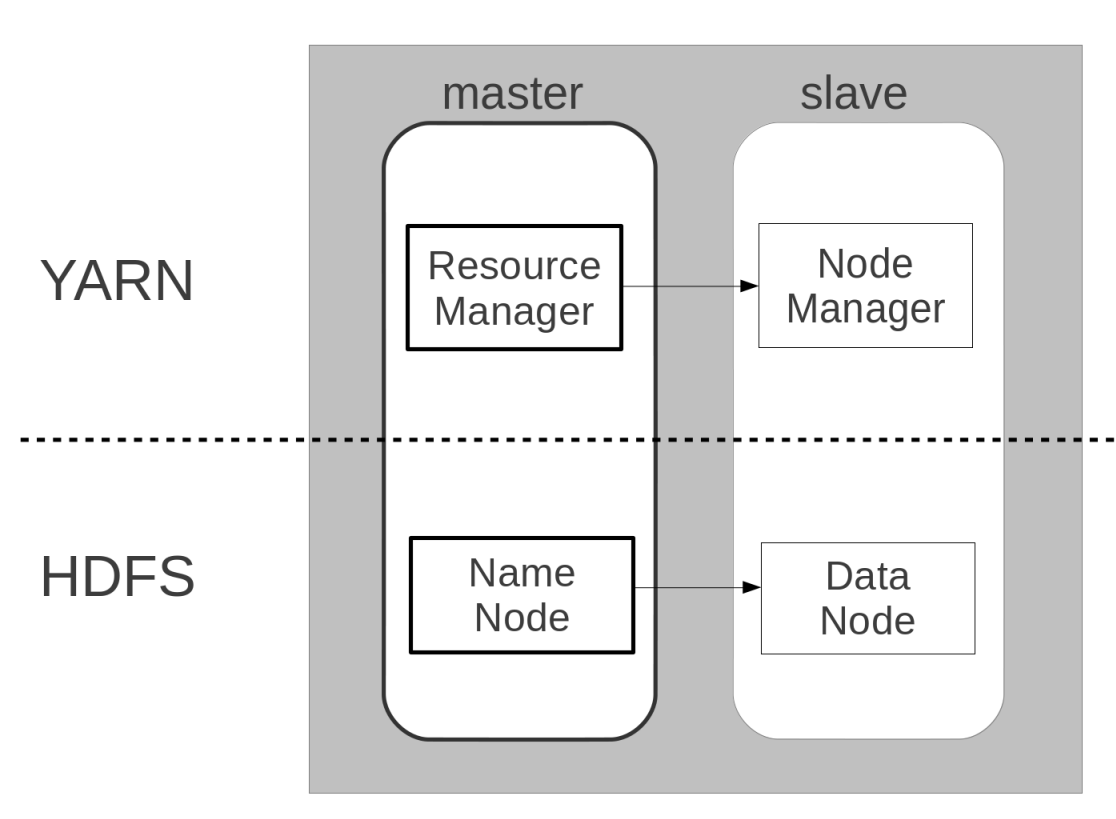
\includegraphics[width=0.7\textwidth]{figuras/Figura08-HadoooArchGeral.png}
\caption{Arquitetura geral do Apache Hadoop}
\label{fig:ArquiteturaHadoop}
\end{figure}

Nesta figura, é possível notar a existência de 4 componentes do \textit{framework}. Os componentes acima da linha pontilhada pertencem ao YARN, sendo o Resource Manager e o Node Manager os serviços mestre e escravo respectivamente. O HDFS é composto pelos componentes abaixo da linha pontilhada, sendo o Name Node e o Data Node os serviços mestre e escravo respectivamente.

\subsubsection{HDFS}
Grande parte do ganho de desempenho oferecido pelo Hadoop decorre do comportamento de levar o processamento até os dados, ou seja, todo processamento é feito com dados locais. Esta abordagem só é possível de ser realizada graças ao HDFS. Dentro do Name Node são mantidas informações de quais partes de quais arquivos estão em cada Data Node, ou seja, todos os arquivos estão divididos num grande HD distribuído e o mestre sabe exatamente quais blocos cada escravo possui. Dessa forma cada nó executa tantos Maps ou Reduces quanto a quantidade de arquivos locais permitir, diminuindo a necessidade de utilizar a rede para transferência de arquivos e deixando-a disponível para ser utilizada para a transferência dos resultados que são os dados já reduzidos. Um problema dessa abordagem é que o Hadoop possui uma latência muito alta, sendo desaconselhável o uso do Hadoop em aplicações críticas ou de tempo real \cite{BookHadoop}. A Figura \ref{fig:ArqHDFS} apresenta um esquema básico da arquitetura do HDFS.

\begin{figure}[!hbtn]
   \centering
   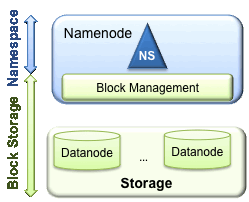
\includegraphics[width=8cm]{figuras/Figura07-HDFS.png}
   \caption{Arquitetura geral do HDFS \cite{HDFS}}
   \label{fig:ArqHDFS}
\end{figure}

\subsubsection{YARN}
Sendo o componente do Apache Hadoop responsável pela execução do \emph{MapReduce}, o YARN realiza tarefas de gerenciamento e execução do processamento. Um dos objetivos do YARN é tornar a tarefa de processamento totalmente independente das tarefas de armazenamento, possibilitando que o \textit{cluster} seja utilizado em conjunto com outras ferramentas que não utilizem o paradigma MapReduce \cite{Vavilapalli}. A Figura \ref{fig:ArqYARN} apresenta um esquema básico da arquitetura do YARN.

\begin{figure}[!hbtn]
   \centering
   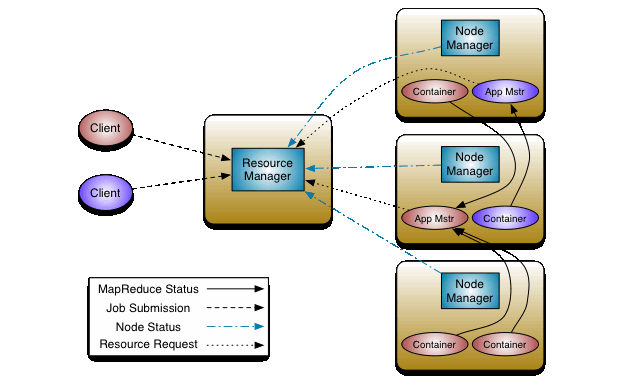
\includegraphics[width=12cm]{figuras/Figura06-YarnArch.png}
   \caption{Arquitetura geral do YARN \cite{YARN}}
   \label{fig:ArqYARN}
\end{figure}

Na imagem é possível observar dois novos componentes do YARN. O primeiro é um componente do Node Manager, possuindo o papel de um escalonador interno de cada aplicação (Application Master - referenciado na imagem como App Mstr), sendo também conhecido por escalonador de tarefas. Considera-se que tarefas sejam uma fração do processamento das aplicações, ou seja, cada tarefa de Map ou Reduce corresponde a uma das divisões que serão processadas em paralelo. É importante não confundir este componente com o escalonador de aplicações, o qual é um componente do Resource Manager e pode ser melhor compreendido com a leitura da Seção \ref{sec:HadSched}. O outro componente presente na figura é o Container, o qual representa uma alocação de recursos em um nó qualquer do \textit{cluster}. A importância do container vem do fato de que todas as tarefas são executadas em uma instância de container.

É importante notar que existem 2 instâncias de Application Master na figura e que elas estão, assim como os clientes e os containers, coloridas de rosa ou roxo para indicar que pertencem à mesma aplicação, ou seja, o cliente rosa lançou uma aplicação que possui o Application Master e mais 3 containers de processamento. Nota-se também que o Resource Manager recebe informações tanto dos clientes quanto dos Node Managers e Application Masters, centralizando todas elas para um controle dos recursos disponíveis.

\subsection{Configuração do ambiente de execução do Hadoops}
Uma característica importante do Hadoop tem relação com sua configuração. Sabe-se que todo sistema necessita de uma configuração por parte de seu administrador, e o Hadoop não é diferente com relação a isso. O Hadoop utiliza uma série de arquivos em cada um dos nós do \textit{cluster} para definir sua configuração. Estes arquivos de configuração são, na verdade, arquivos XML compostos por parâmetros de configuração e valores que influenciam o comportamento do \textit{framework} no \textit{cluster}. Para conhecimento, esses arquivos são: \textit{core-site.xml, yarn-site.xml, mapred-site.xml} e \textit{hdfs-site.xml}. Cada um destes arquivos possui propriedades de um serviço do Hadoop, como exemplo o arquivo \textit{hdfs-site.xml} é responsável pela configuração do HDFS na máquina em questão. 

É importante salientar que para a execução distribuída, ao menos algumas propriedades mais simples dos arquivos de cada nó, seja este mestre ou escravo, devem ser configuradas. No caso do administrador desejar fazer uma configuração mais específica de cada nó escravo ele deverá editar as propriedades nos arquivos de cada um dos nós. Caso o administrador não queira configurar os nós escravos, eles irão executar com base nos valores \textit{default}, contudo esta decisão irá, provavelmente, afetar o desempenho do \textit{cluster} devido à má configuração.

\section{MapReduce}
O paradigma de programação MapReduce é, geralmente, associado com implementações que processam e geram grandes conjuntos de dados. Neste paradigma, todo processamento é dividido em duas etapas, a etapa de Map e a de Reduce, originárias das linguagens funcionais. Como consequência da divisão em duas etapas, o resultado da primeira é a entrada da segunda e esta transferência de dados é baseada em de pares de chave e valor, o que torna possível expressar uma vasta gama de tarefas reais por meio deste paradigma \cite{Dean}.

O \textit{work-flow} padrão de uma aplicação MapReduce inicia com a entrada de dados, que será dividida em \textit{n} partes e cada parte será processada individualmente por uma tarefa Map. O resultado das tarefas Map já será na forma de pares chave e valor, que serão passados como entrada para as tarefas de Reduce. Por sua vez, as tarefas de Reduce irão receber todos os pares com determinada chave e aplicar um algoritmo sobre os pares, fornecendo uma saída inteligível \cite{BookHadoop}.

%TODO citação
A naturalidade do paralelismo deste paradigma, torna a programação da aplicação mais simples. Ao utilizar o paradigma do MapReduce o programador deve apenas pensar em uma solução que siga o \textit{work-flow} do paradigma, e o parelelismo será inerente.

\section{ZooKeeper}
O ZooKeeper é um projeto da Apache e fornece ferramentas eficientes, confiáveis e tolerantes à falha para a coordenação de sistemas distribuídos \cite{Hunt2010}. Inicialmente, o ZooKeeper foi implementado como um componente do Hadoop e virou um projeto próprio conforme cresciam suas funcionalidades e sua utilização em outras aplicações. 

A arquitetura utilizada no ZooKeeper é a de cliente-servidor, sendo o servidor o próprio ZooKeeper (chamado de \textit{ensamble}), enquanto a aplicação que o está utilizando assume o papel de cliente. A maneira como os clientes interagem depende da aplicação.

Os dados do ZooKeeper ficam armazenados em \textit{zNodes}, abstrações que podem ser tanto um \textit{container} de dados quanto de outros \textit{zNodes}, e formam um sistema de arquivos hierárquico que pode ser comparado à estrutura de uma árvore. Para garantir a consistência deste sistema de arquivos o ZooKeeper utiliza operações de escrita linearizáveis, as quais são obrigatoriamente processadas pelo servidor líder que é, então, encarregado de propagar as mudanças para os demais participantes do \textit{ensamble} \cite{Pham}.

Um dos principais recursos do ZooKeeper são os \textit{Watchers}, interfaces providas pelo \textit{framework} que permitem aos clientes monitorarem certos \textit{zNodes}. Quando um \textit{Watcher} é registrado como monitor de um \textit{zNode}, ele pode ser configurado para monitorar a alteração dos dados do \textit{zNode}, a criação/remoção de \textit{zNodes} filhos, ou ainda para qualquer tipo alteração no \textit{zNode} e seus filhos. Quando um \textit{zNode} sofre uma alteração que o \textit{Watcher} está monitorando uma \textit{callback} é disparada para que o cliente faça o processamento desejado \cite{HadoopBook}.

No âmbito deste trabalho, os serviços do ZooKeeper são utilizados para monitorar as informações de contexto coletadas nos nós escravos e transmiti-las para o escalonador. Sendo que a comunicação é feita através de processos que atualizam e monitoram o conteúdo de \textit{zNodes}.


%-------------------------------------------------------------------

\section{Escalonadores para o Hadoop}
\label{sec:HadSched}
Apesar de existirem dois níveis de escalonamento no Hadoop, escalonamento de aplicações e de tarefas, este trabalho influencia apenas o escalonamento de aplicações. O escalonador de aplicações gerencia qual será a primeira aplicação a receber um \textit{container} para seu escalonador de tarefas e quais serão os escalonadores de tarefa que receberão recursos para execução \cite{BookHadoop}. O Hadoop já inclui alguns escalonadores que oferecem maneiras diferentes para a realização do escalonamento de aplicações. Para alterar o escalonador utilizado é necessário alterar uma propriedade no arquivo \textit{yarn-site.XML} e reiniciar o Resource Manager.

Dentre os escalonadores incluídos no Hadoop, o mais simples é o Hadoop Internal Scheduler que utiliza o algoritmo FIFO e tem boa performance em \textit{clusters} onde não existe competição por recursos. Este escalonador suporta até 5 níveis de prioridade, porém a decisão da próxima aplicação a ser executada sempre levará em consideração a hora de submissão.

Um pouco mais complexo que o Internal Scheduler, o Fair Scheduler é utilizado principalmente para o processamento de lotes de aplicações pequenas e rápidas, opera baseado em um escalonamento de dois níveis e possui o objetivo de realizar uma divisão justa dos recursos. O primeiro nível realiza o escalonamento na forma de filas para cada usuário ativo, dividindo os recursos do cluster igualitariamente entre as filas. Enquanto isso, o segundo nível realiza o escalonamento dentro de cada fila da mesma forma que o Internal Scheduler \cite{FairScheduler}. 

A terceira opção, e também o padrão do Hadoop nas últimas versões, é o Capacity Scheduler, o qual foi projetado para a utilização compartilhada do Hadoop e busca a maximização do \textit{throughput} e da utilização do \textit{cluster}. Seu funcionamento baseia-se em garantias mínimas de capacidade para os usuários, ou seja, qualquer usuário terá sempre uma garantia mínima de recursos para utilização. Porém quando algum usuário está com seus recursos ociosos o escalonador repassa a capacidade deste usuário  para aqueles que estão utilizando o \textit{cluster}. Esta estratégia fornece elasticidade com um bom custo benefício, uma vez que diferentes organizações possuem diferentes horários de pico para o processamento de informações. Este escalonador é capaz de rastrear os recursos registrados no Resource Manager, embora esta informação pode não ser consistente com a realidade, e monitorar quais deles estão livres e quais estão sendo utilizados pelo \textit{framework} \cite{CapacityScheduler}.

A existência destes escalonadores adiciona flexibilidade no gerenciamento do \textit{framework}. Apesar disso, os escalonadores disponíveis não detectam nem reagem à dinamicidade e heterogeneidade do ambiente. Para a utilização do Hadoop em ambientes pervasivos é necessário que exista uma capacidade de adaptação neste componente.




%-------------------------------------------------------------------

\section{Trabalhos Relacionados}
%TODO adicionar os novos trabalhos que não existiam no TG
Existem outras implementações de escalonadores além dos 3 escalonadores já inclusos no Hadoop, nas quais é possível identificar diversas propostas de adaptação. Cada proposta possui métodos e objetivos específicos, tornando um estudo sobre estas implementações interessante como ponto de partida para a proposta deste trabalho. Logo, buscou-se identificar quais técnicas foram mais utilizadas e quais os tipos de adaptação mais explorados nestes escalonadores. A seguir encontram-se os trabalhos relacionados e um breve resumo sobre a proposta, método e objetivos esperados com a adaptação.


Os autores do escalonador CASH (\emph{Context Aware Scheduler for Hadoop} - Escalonador Sensível ao Contexto para o Hadoop) \cite{CASH} têm o objetivo de melhorar o rendimento geral do \emph{cluster}. O trabalho utiliza a hipótese de que grande parte das aplicações são periódicas e executadas no mesmo horário, além de possuírem características de uso de CPU, rede, disco etc. semelhantes. O trabalho ainda leva em consideração que com o passar do tempo os nós tendem a ficar mais heterogêneos. Baseados nestas hipóteses e com objetivo de melhorar o desempenho geral, foi implementado um escalonador que classifica tanto as aplicações como as máquinas com relação ao seu potencial de CPU e E/S, podendo então distribuir as aplicações para máquinas que tem uma configuração apropriada para sua natureza.

No trabalho \textit{A Dynamic MapReduce Scheduler for Heterogeneous Workloads} (Um Escalonador de MapReduce Dinâmico para Cargas de Trabalho Heterogêneas) \cite{DMRSHW}, os autores utilizam a técnica de classificar as aplicações e máquinas de acordo com a quantidade de E/S ou CPU. E assim como no CASH, o principal objetivo é a melhora de rendimento no \textit{cluster}. Uma das diferenças, no entanto, é que esta implementação utiliza um escalonador com três filas.

Semelhante às propostas anteriores, a proposta COSHH (\textit{A Classification and Optimization based Scheduler for Heterogeneous Hadoop Systems} - Um Escalonador Baseado em Classificação e Otimização para Sistemas Heterogêneos do Hadoop) \cite{COSHH} utiliza a classificação das aplicações e máquinas em classes e busca por pares que possuam a mesma classe. Esta busca é feita por um algoritmo que reduz o tamanho do espaço de busca para melhorar o desempenho. O objetivo desta solução é a melhora do tempo médio em que as aplicações são completadas, além de oferecer um bom desempenho quando utilizando somente a fatia mínima de recursos e, ainda, proporcionar uma distribuição justa.
%O artigo não informa quais informações são utilizadas para a classificação. 

O escalonador LATE (\textit{Longest Approximation Time to End} - Aproximação do Tempo de Término mais Longo) \cite{LATE}, utiliza como informação de contexto o tempo estimado de término da tarefa com base em uma heurística que faz a relação de tempo decorrido e do \textit{score} -- um valor que indica quanto do processamento já foi feito. Essa informação também é utilizada para gerar um limiar que indique quando a lentidão de uma tarefa indica sintomas de erros e a partir desta informação iniciar uma tarefa especulativa em outra máquina possívelmente mais rápida. Este trabalho possui o objetivo de reduzir o tempo de resposta em \textit{clusters} grandes que executam muitas aplicações de pequena duração.

Outro trabalho que utiliza a ideia de mensuração do progresso de uma tarefa é o SAMR (\textit{A Self-adaptative MapReduce} - MapReduce Auto Adaptativo) \cite{SAMR}, nesta implementação a informação de contexto é referente ao cálculo do progresso de uma tarefa com objetivo de identificar se é o lançamento de uma tarefa especulativa é necessário ou não. Uma diferença desta solução é com relação ao cálculo do progresso, o qual varia de acordo com informações do ambiente em que a tarefa está executando. O principal objetivo do trabalho é a redução do tempo de execução das tarefas. As informações do ambiente utilizadas para a tomada de decisão consistem de informações históricas contidas em cada nó, e a decisão é tomada após um ajuste do peso de cada estágio do processamento.


A proposta dos autores do \textit{Quincy} \cite{Quincy} difere-se de todos os outros trabalhos, pois possui um escopo muito maior e visa tanto o \textit{Hadoop} como outras ferramenas. O trabalho possui como objetivo a melhora do desempenho geral de um \textit{cluster}, e utiliza a distribuição de recursos como informação de contexto para alcançá-lo. A contribuição do trabalho é uma modificação da maneira tradicional de tratamento da distribuição dos recursos. A solução proposta mapeia os recursos em um grafo de capacidades e demandas, para então calcular o escalonamento ótimo a partir de uma função global de custo.

A proposta \textit{Improving MapReduce Performance through Data Placement in heterogeneous Hadoop Clusters} (Melhorando o Desempenho do MapReduce em Clusters Heterogêneos com Hadoop Através da Localização dos Dados) \cite{IMRPDPHHC}, busca melhorar o desempenho de aplicações CPU-bound através da melhor distribuição destes dados. Esta solução utiliza principalmente a localidade dos dados como informação para tomada de decisões. O ganho de desempenho é dado pelo rebalanceamento dos dados nos nós, deixando nós mais rápidos com mais dados. Isso diminui o custo de tarefas especulativas e de transferência de dados pela rede.

Outra proposta que busca um rebalanceamento de carga é \cite{Sandholm}, porém esta utiliza-se de uma abordagem diferente. Neste trabalho o rebalanceamento de carga é alcançado através de um sistema baseado na lei de oferta e demanda, o qual permite a cada usuário influenciar diretamente o escalonamento por meio de um parâmetro chamado taxa de gastos. Este parâmetro indica qual a prioridade da aplicação, sendo que, em horários de maior concorrência a taxa de gasto será maior. O principal objetivo deste trabalho é permitir um compartilhamento de recursos dinâmico baseado em preferências configuradas pelos próprios usuários.


Nota-se que no geral as propostas de melhora da adaptabilidade apresentadas pelos trabalhos utilizam principalmente a técnica de rebalanceamento de carga entre nós de diferentes capacidades. Ainda, é possível notar que os trabalhos, em sua maioria, seguem três opções:

\begin{enumerate}
	\item Classificação dos nós e das aplicações de acordo com sua capacidade (CPU ou E/S) seguido de um algoritmo que delega aplicações para nós do mesmo tipo;
	\item Modificação da tomada de decisão sobre o lançamento ou não de uma tarefa especulativa através de novas heurísticas;
	\item Redistribuição dos dados para que eles fiquem em nós mais rápidos.
\end{enumerate}

Ainda que a opção 3 assemelhe-se com a opção 1, é importante diferenciar a natureza delas. Enquanto a opção 1 classifica os nós em diversas categorias, a opção 3 apenas delega mais dados, e consequentemente mais tarefas, aos nós mais rápidos. Embora pareça uma solução mais simples ela evita transferência de dados pela rede, o que aconteceria caso a divisão dos dados para os nós fosse igualitária.

%TODO Changlong Li \cite{Li}
Embora não relacionado com escalonamento, o trabalho \cite{Li} propõe uma ferramenta de auto configuração que em partes assemelha-se com a proposta deste trabalho. Entretanto, a proposta de Li é baseada em aprendizagem de máquina para a auto configuração de alguns parâmetros chave do Hadoop e apresenta execuções até 10 vezes mais rápidas após a otimização dos parâmetros; enquanto a proposta deste trabalho busca melhorar a informação disponível para o escalonador.
\newpage

\section{TABELA}
%Tabela dos casos
\begin{table}[!h]
	\centering
	\begin{tabular}{|p{3.0cm}|p{6.0cm}|p{6.0cm}|}
		\hline
		Situação & Default & Trabalho \\
		\hline
		Falha nó (morto) & perde tasks (precisa reiniciar quando tiver recursos) e desregistra NM (diminui recursos) & Idem default\\
		\hline
		Novo nó (registro) & registar novo NM. Aumenta recursos e escalona tasks que estavam esperando & Idem default\\
		\hline
		Nó inicia compartilhamento (- recurso) & \textbf{não reage}, continua alocando containers como se estivesse tudo disponível & \textbf{diminui o recurso do nó. Não afeta containers já alocados, mas só irá alocar quando possuir recurso disponível}\\
		\hline
		Nó termina compartilhamento (+ recurso) &\textbf{não reage}, se o nó já estava configurado para utilizar apenas uma parte ele não irá passar a ocupar todos recursos & \textbf{aumenta o recurso do nó. Inicia nova rodada de escalonamento, é como se um novo nó entrasse}\\
		\hline
		Cluster heterogêneo & tem que alterar as propriedades dos recursos no XML de todos escravos refletindo as configurações dos nós. Caso contrário existirão nós sobrecarregados ou subutilizados. & Cada nó tera a informação correta. Ganho de desempenho por não sobrecarregar nem subutilizar.\\
		\hline
		
	\end{tabular}
	\caption{tabela de casos}
	\label{tab:memory allocation}
\end{table}

%Tabela dos testes
\begin{table}[!h]
	\centering
	\begin{tabular}{|p{2.5cm}|p{3.5cm}|p{4.5cm}|p{4.0cm}|}
		\hline
		Teste & Representa.. & Metodologia & Ponto fraco\\
		\hline
		Enganar escalonador para achar que tem mais recursos & cluster compartilhado no momento do início da utilização por outro usuário & inicia x nós com recursos informados dobrados, atualiza durante a primeira leva de containers para valor correto & desta forma é necessário utilizar apenas x/2 nós em relação ao caso A. Pode confundir com um caso de falha de nós\\
		\hline
		Nó compartilhado de verdade com informação errada (overload)& cluster compartilhado no momento do início da utilização por outro usuário & reduzir algum recurso de forma que fique indisponível durante a execução. Opções: baloon(MV) - memória, thread - cpu & como garantir que a memória/cpu estará realmente indisponível? quantidade de trabalho extra para realizar o teste\\
		\hline
		Enganar escalonador para achar que tem menos recursos & cluster compartilhado no momento do fim da utilização por outro usuário & inicia x nós com recursos informados de x/2, atualiza durante a primeira leva de containers para valor correto & Caso muito improvável, administrador configura o cluster para o Hadoop utilizar apenas uma parte dos recursos dos nós.\\
		\hline
		Nó compartilhado de verdade com informação errada (underload)& cluster compartilhado no momento do fim da utilização por outro usuário & reduzir algum recurso de forma que fique indisponível antes do início e torná-lo disponível durante execução. Opções: baloon(MV) - memória, thread - cpu & como garantir que a memória/cpu estará realmente indisponível? quantidade de trabalho extra para realizar o teste\\
		\hline
		Teste completo inicia e termina compartilhamento em momentos diferentes durante execução & cluster compartilhado & Inicia com 75\% disponível, reduz recurso durante execução de forma que fique sobrecarregado e aumenta recurso durante execução de forma que fique sub utilizado. Opções: {várias combinações} possíveis de \% & Só é possível fazer sem enganar o cluster. Precisa dos outros testes com controle de recursos funcionando\\
		\hline
	\end{tabular}
	\caption{tabela de testes}
	\label{tab:memory allocation2}
\end{table}
\chapter{Métodos e Desenvolvimento}
Este capítulo descreve as etapas de desenvolvimento e as metodologias empregadas neste trabalho. Buscaram-se estratégias sem intrusão ou grandes modificações nas políticas de escalonamento já implementadas pelo \textit{framework}. Na Seção \ref{sec:exp-prelim} encontram-se informações sobre alguns experimentos preliminares realizados com intuito de obter melhor compreensão dos mecanismos de escalonamento e funcionamento interno do Hadoop. Nas Seções \ref{sec:collector} e \ref{sec:zookeeper} são apresentados em maior detalhe, os coletores de contexto e a ferramenta de comunicação distribuída, utilizados neste trabalho, respectivamente. 

%-------------------------------------------------------------------

\section{Understanding Apache Hadoop internals}
\label{sec:grafo}
Aiming to insert context-awareness on a scheduler, it is necessary that the architecture of Apache Hadoop is comprehended. This stage of the project had the objective to identify the dependencies between the classes, besides which classes would be necessary to implement and how would this implementation take place.

Since a working scheduler requires many abstract classes and interfaces to be implemented, it is a good practice to know the origins of these components and how they influence the final class. Also, through the architecture study  it is possible to identify the resources supported by the framework, making it possible to decide the scheduling strategies.

Two methods were used in order to study the architecture. The first method consisted on source code study, while the second method was a study of the state machines that dictate the functioning of Resource Manager. This stage was planned aiming  the identification of all components inside a scheduler, since the implemented interfaces and abstract classes to the scheduling criteria and how these are applied on available schedulers.

\subsection{Code structure and class diagrams}

Given the framework's complexity, it was decided to use an IDE on the execution of the first method, in this case the chosen IDE was IntelliJ IDEA \cite{IDEA}. Once the study was finished, it was possible to generate a series of class diagrams. The generated diagrams were used in conjunction with HortonWorks  Diagram in order to make the understanding of the whole YARN framework easier.

The first diagrams used in this step were the ResourceManager and NodeManager component diagrams, which provided a better high level understanding of the components that compose the ResourceManager and NodeManager.

The figure \ref{fig:RMHorton} illustrates the high level view of the ResourceManager. It is possible to note many modules which doesn't matter to the context of this work, such as: Security, DelegationTokenRenewer, among others. Even so, the notion this figure passes has a high value to the understanding.

\begin{figure}[hbtn]
   \renewcommand{\figurename}{Figure}
   \centering
   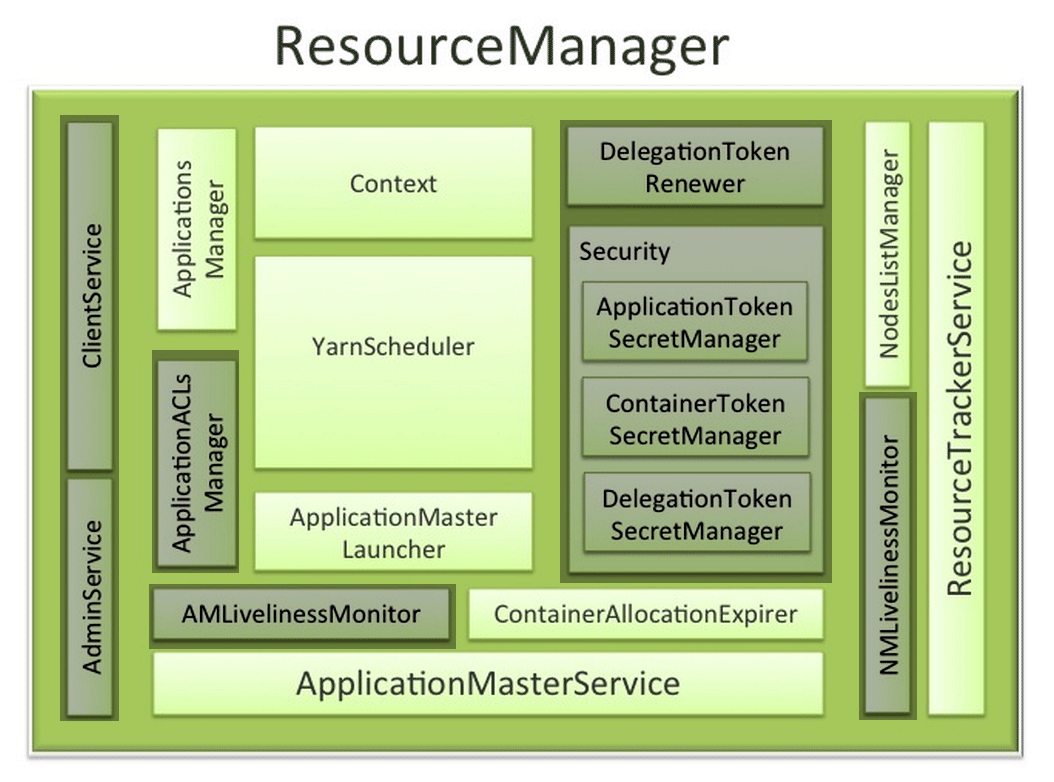
\includegraphics[width=15cm]{figuras/Figura14-RMHorton.png}
   \caption{ResourceManager Component Diagram \cite{HortonRM}}
   \label{fig:RMHorton}
\end{figure}

The ResourceManager is the master that arbitrates all the available cluster resources and thus helps manage the distributed applications running on the YARN system. It works together with the per-node NodeManagers (NMs) and the per-application ApplicationMasters (AMs) \cite{HortonRM}.

Except the scheduler itself, there are other components of fundamental importance to the scheduling process. Like the ApplicationsManager, which manages all the submitted applications. The ApplicationsManager component not only has a list of submitted applications, but also has information about all the completed applications and is able to provide this through either web UI or command line.

Another important component is the ApplicationMasterLauncher, that will be responsible to create the application specific ApplicationMaster, everytime an application is submitted. Another task left to the ApplicationMasterLauncher component is the deletion of ApplicationMaster when the application has finished, either normally of forcefully.

The ApplicationMaster itself is a concept that makes YARN completely different than the previous Hadoop versions. It is a key component on MapReduce tasks execution because it has one instance for every application being executed, making the ApplicationMaster the component responsible for the execution and monitoring of the containers and their resource consumption. Therefore, it has to communicate with the ResourceManager in order to ask and report the status and progress of its monitored containers.

It is through ApplicationMaster that YARN can achieve better scalability, since it takes some of the processing usually delegated to the Scheduler and ResourceManager components. One of the key tasks that was transferred to the ApplicationMaster is the fault tolerance. It is the ApplicationMaster that will decide when and/or if a speculative task is necessary and beneficial. Thanks to this shift in the responsibilities and the ApplicationMaster being a per-application manager, the cluster scaling potential is improved through the removal of a possible bottleneck. 

Another crucial component to the present work is the ResourceTrackerService, that is responsible for the communication with the NodeManagers. This is the component that answers to the RPC calls, whenever a node wants to register with the RM, send a heartbeat, or many other tasks, this is the component that will be used. The node capacity is also passed on the registration of a node with the RM, this process of registration will store the node's information in the NodesListManager. The second component is a collection of all the nodes, both the valid and the decomissioned ones.

Finally, the Scheduler follows the same pattern as regular scheduler, comparing requests, availabilities and then granting the resources based on some heuristic. However, most Hadoop schedulers use queues in order to help the task of managing the users and application submitted.

The other high level view that interests this work is the NodeManager. Just as the ResourceManager counterpart, even having some irrelevant modules presented in the figure \ref{fig:NMHorton}, it facilitates the understanding of the service in a high level. Having a high level understanding is necessary in order to understand how the two services will interact.

\begin{figure}[hbtn]
   \renewcommand{\figurename}{Figure}
   \centering
   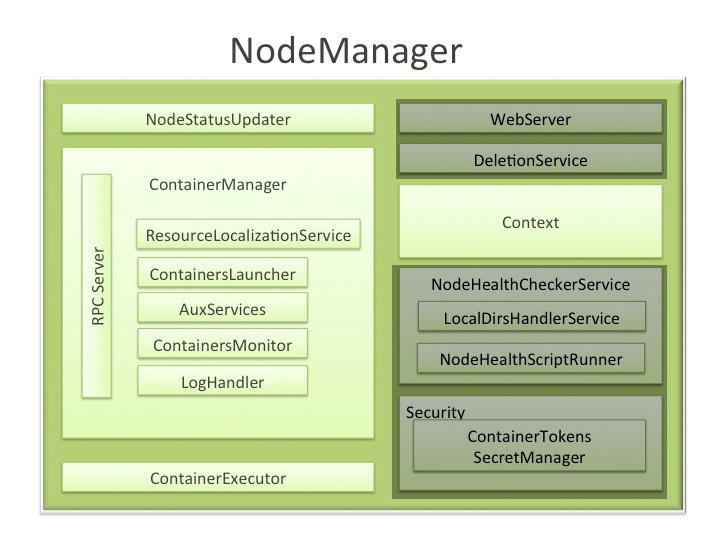
\includegraphics[width=15cm]{figuras/Figura15-NMHorton.png}
   \caption{NodeManager Component Diagram \cite{HortonNM}}
   \label{fig:NMHorton}
\end{figure}

Each slave will have a NodeManager instance running, which is the local manager. This service main responsibility is keeping his information updated on the ResourceManager, but it has other attributions like managing the containers, monitoring the resource usage, monitoring node health, among others.

One key component is the NodeStatusUpdater, which will be responsible for the registration with the ResourceManager, it is through registration that the ResourceManager will be informed about the resources of a given node, making this component vital for the success of the approach in this work. Also, after the initial registration this component is expected to maintain the communication with the ResourceManager in order to provide updates on containers launched, running or completed.

The largest component in the figure, the ContainerManager is as important as its size implies. With help from its sub-components, the ContainerManager has the hard but extremely necessary task of monitoring containers and informing whatever component needs this information. There are several ContainerManager sub-components, they are: RPC server, ResourceLocalizationService, ContainersLauncher, AuxServices, ContainersMonitor and LogHandler. Some like the ResourceLocalizationService is of vital importance to the MapReduce tasks, as it downloads the files that will be used on the tasks' execution, but won't interfere in this work's context.

The next diagram used to better understand the architecture was the scheduler components class diagram, which provided a helped to view classes related to the scheduling process. The Scheduler Components Class Diagram can be visualized in the figure \ref{fig:SchedCD}.

\begin{figure}[hbtn]
   \renewcommand{\figurename}{Figure}
   \centering
   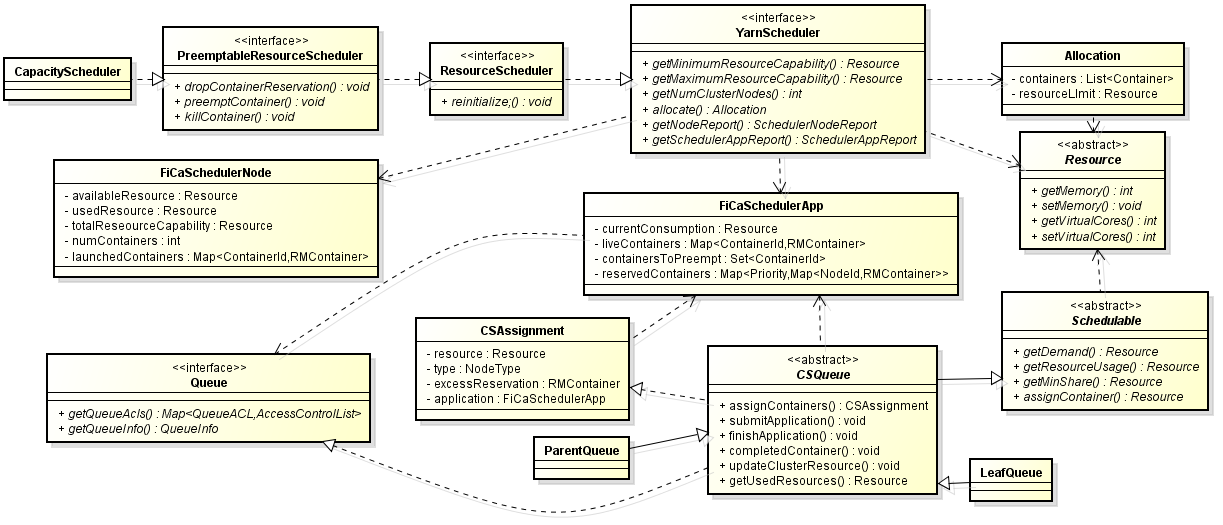
\includegraphics[width=15cm]{figuras/Figura01-ClassDiagram.png}
   \caption{Class Diagram with the main CapacityScheduler classes}
   \label{fig:SchedCD}
\end{figure}

Following is a description of the main components that compose the CapacityScheduler:
\begin{itemize}
	\item Schedulable: an abstract class that represents an entity capable of launching either a job or a queue, it offers a simple interface whereby the algorithms can be applied either inside a queue as well as several queues.
	\item Queue: an interface that enables the basic control of all the queues in the scheduler. Possessing methods to allow reading of the queue info, and also queue management.
	\item PreemtableResourceScheduler: another interface that allows the preemption of resources, through the scheduler.
	\item Resource: an abstract class responsible for modelling the resources capable of being use, which at this moment are only memory and core count.
	\item FiCaSchedulerNode and FiCaSchedulerApp: representations of the node and application, provides vital information about the structures. Uses a lot of the components present on the next Class Diagram.
\end{itemize}

Another key class diagram to the context of this work was the diagram that would represent three very important components, the RMContainer, RMNode and RMApp/RMAppAttempt. All of these components represents fundamental parts on understanding how this work has impacted the scheduling. RMContainer is the name given to the reservations of resources, making it also responsible for the task execution. RMNode is the representation of a whole NodeManager to the scheduler, and is through it that the scheduler will get access to the NodeManager real resource capacity. RMApp and RMAppAttempt represents the applications sent to the scheduler. This diagram is represented in the figure \ref{fig:RMComponents}.

\begin{figure}[hbtn]
   \renewcommand{\figurename}{Figure}
   \centering
   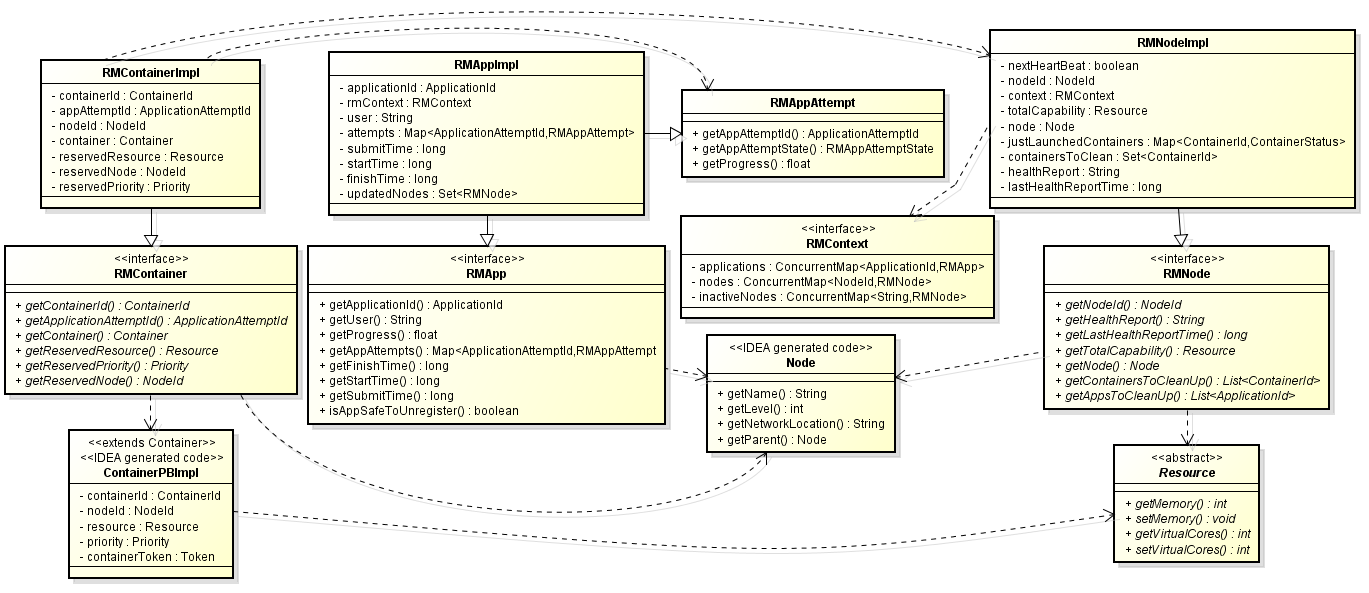
\includegraphics[width=15cm]{figuras/Figura13-RMComponents.png}
   \caption{Class Diagram with the main RM components}
   \label{fig:RMComponents}
\end{figure}

\subsection{State machines}

The second method was executed through an option offered by the Maven tool, in which it is possible to generate graphs that represents the Resource Manager and Node Manager state machines. Through analysis of the graphs it is possible to identify the life cycle of some key components, such as RMContainers, RMNodes and RMApplications. 

The importance of RMContainers, RMNodes and RMApplications may be overlooked until further analysis of source code and state machines at the same time. It is not a coincidence that all the components have a RM, referencing ResourceManager, in their names. In a brief explanation, RMNodes have all resource and other static information concerning a given NodeManager. RMContainers are the structures that represent the reservation of resources and also responsible for the processing. Finally, the RMApplication is the component that provides ResourceManager a way to access application status, reports and updates. All state machines and a more thorough explanation can be found on \autoref{chap:ApendA}.

%-------------------------------------------------------------------

\section{Understanding Hadoop allocation pattern}
\label{sec:alloc}
In order to improve Hadoop resource utilization and change the resource allocation behavior, it was necessary to understand how the allocation is made. That implies knowing and understanding the whole process of requisition and grant of resources, which is essentially the scheduling. After the experiments made with the objective of understanding this process, it was possible to identify which parameters influenced and how much impact would these parameters have once they were changed.

Once a quick research on official documentation and the parameters which can be set on XML files was made, it was found that there are five parameters that influence the allocation pattern for each resource. These parameters can be roughly divided into three classes: application request, cluster configuration towards containers and cluster configuration towards ApplicationMaster (AM). All of these parameters have default values in case the application did not set a request value or the cluster administrator did not set them properly on configuration files.

The application request parameters are set through the JobConf class when the user is coding his MapReduce job. If the parameters are not set at this time, the cluster will use the properties \textit{mapreduce.map.memory.mb} and \textit{mapreduce.reduce.memory.mb} either at the \textit{mapred-site.xml} or \textit{mapred-default.xml}, following default Hadoop behavior towards settings in the xml files. The default behavior is: if the properties are set in any \textit{*-site.xml} file that's the value they will assume, otherwise the values will be taken from \textit{*-default.xml} file.
The default value for properties \textit{mapreduce.map.memory.mb} and \textit{mapreduce.reduce.memory.mb} is 1024.

The cluster configuration towards containers is composed by four parameters, these parameters express the floor and ceiling of valid allocations. The floor limit parameters receive their values from the properties \textit{yarn.scheduler.minimum-allocation-mb} related to the memory and \textit{yarn.scheduler.minimum-allocation-vcores} related to the cores, while the ceiling limit parameters receive their values from properties \textit{yarn.scheduler.maximum-allocation-mb} and \textit{yarn.scheduler.maximum-allocation-vcores}. All properties will follow the default Hadoop behavior towards settings in XML files. These four parameters are related to two variables in the source code, which are named \textit{minimumAllocation} and \textit{maximumAllocation}, which represents the floor and ceiling limit respectively. 
The default value for \textit{yarn.scheduler.minimum-allocation-mb} is 1024 and the default value for  \textit{yarn.scheduler.minimum-allocation-vcores} is 1. The default values concerning the ceiling properties is 8192 for \textit{yarn.scheduler.maximum-allocation-mb} and 32 for \textit{yarn.scheduler.maximum-allocation-vcores}.

The only parameter left is the AM request, this request will be the same for every application submitted to the cluster and cannot be configured through JobConf. This parameter will receive it's value from properties \textit{yarn.app.mapreduce.am.resource.mb} related to the memory and \textit{yarn.app.mapreduce.am.resource.cpu-vcores} related to the cores, also following the default Hadoop behavior. The default value of the parameter \textit{yarn.app.mapreduce.am.resource.mb} is 1536, and, the default value of the parameter \textit{yarn.app.mapreduce.am.resource.cpu-vcores} is 1.

\subsection{Experiment}
In order to understand how the allocation process is made an experiment was performed. The experiment was made aiming to understand how the RM allocates memory for applications given requisition and minimum/maximum parameters changes. It consisted in altering some of the parameters and analysing the resultant behavior. As the AM request is the same across the cluster, it was excluded from the experiment. The reason being that different applications would have the same amount requested by the AM and it's behavior follows the same pattern as the other requests, which are easier to manipulate.

\subsubsection{Employed methods, procedures and scenarios}
The experiment was performed in a cluster deployed on Grid'5000 environment. The cluster had five nodes, one master and four slaves, each node having the following configuration: 2 CPUs AMD@1.7GHz, 12 cores/CPU and 47GB RAM. All nodes were running an Ubuntu-x64-1204 standard image, having Sun JDK 1.7 installed. The Hadoop distribution was the 2.2.0 YARN version.

The procedure chosen as data acquisition method was the Hadoop Log System. The reason for such a choice was that Hadoop Log System is, by default, enabled in the INFO level and using the INFO level would be possible to insert small entries and extract useful information in real time.

Following there is a brief description of the four scenarios used in the experiment:

\begin{itemize}
	\item \textbf{Default scenario}: no parameter was changed.
	\item \textbf{Requisition higher than maximum}: the application requested an amount of memory higher than the cluster maximum allocation parameter. The changed value was the maximum allocation memory. The minimum was also changed for consistency reasons.
	\item \textbf{Requisition smaller than minimum}: the application requested an amount of memory smaller than the cluster minimum allocation parameter. The changed value was the minimum allocation memory.
	\item \textbf{Requisition inside range}: the application requested an amount of memory inside the cluster valid range. The changed values were the minimum allocation memory and requisition from both map and reduce.
\end{itemize}

\subsubsection{Results and interpretation}

The results from the scenarios can be analysed on the table \ref{tab:memory allocation}.

\begin{table}
	\renewcommand{\figurename}{Table}
	\centering
	\begin{tabular}{|l|c|c|c|c|}
		\hline 
		Parameters & Default & Higher & Smaller & Inside\\ 
		\hline 
		Map Memory Requisition (MB) & 1024 & 1024 & 1024 & 3456\\ 
		\hline 
		Reduce Memory Requisition (MB) & 1024 & 1024 & 1024 & 3712\\ 
		\hline 
		Minimum Memory (MB) & 1024 & 512 & 2048 & 512\\ 
		\hline 
		Maximum Memory (MB) & 8192 & 768 & 8192 & 8192\\ 
		\hline 
		Map Memory Allocation (MB) & 1024 & ERROR & 2048 & 3584\\
		\hline
		Reduce Memory Allocation (MB) & 1024 & ERROR & 2048 & 4096\\ 
		\hline 		
	\end{tabular}
	\caption{RM memory allocation pattern experiment results}
	\label{tab:memory allocation}
\end{table}

%\begin{figure}[!hbtn]
%   \centering
%   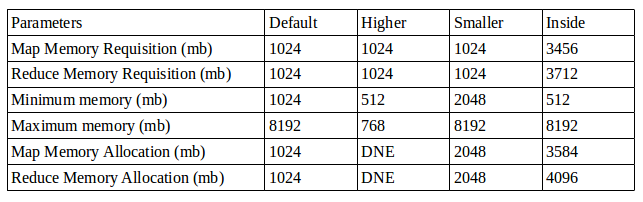
\includegraphics[width=15cm]{figuras/Figura09-allocation.png}
%
%\end{figure}

Because of the experiment, it was possible to detect that Hadoop allocation pattern differs a bit from usual. Unlike usual pattern in which if a request is inside the minimum and maximum range, the amount granted is equal to the request, the requests on Hadoop will pass through a small set of calculations in order to determine how much memory will be granted.

The figure \ref{fig:fluxoAllocation} portraits the  flow of operations executed by the Hadoop in order to determine the granted resources.

\begin{figure}[!hbtn]
   \renewcommand{\figurename}{Figure}
   \centering
   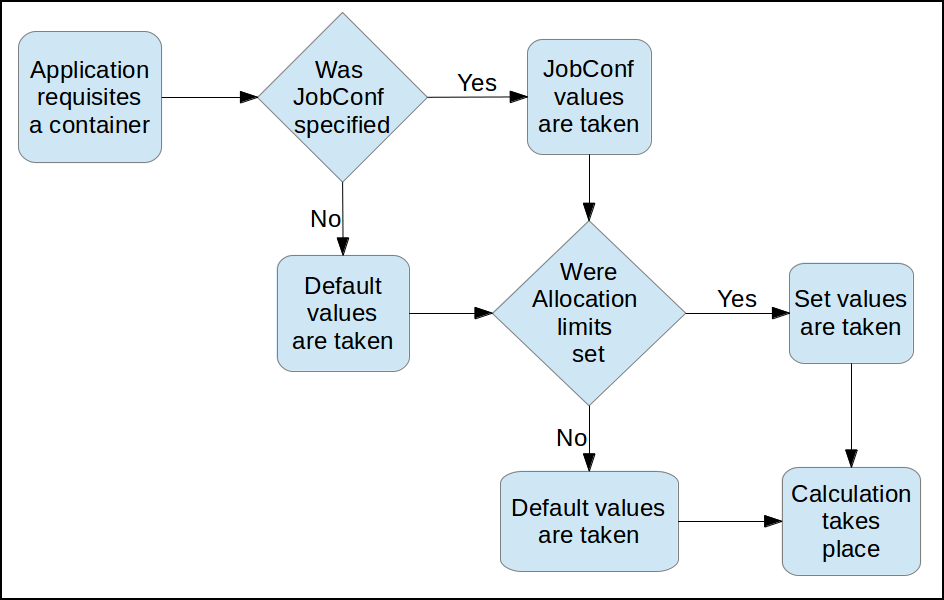
\includegraphics[width=15cm]{figuras/Figura18-allocflow.png}
   \caption{Flow of operations for resource granting}
   \label{fig:fluxoAllocation}
\end{figure}

The default scenario just demonstrates how Hadoop allocation will behave in case there are no interventions.

The second scenario shows what happens if the application requests a value higher than the maximum. The output is an error message and the job execution is aborted.

The third scenario shows what happens if the application requests a value smaller than the minimum. The cluster grants the minimum allowed.

The fourth scenario shows a case in which the requests are inside the valid range but although the requests were similar, the resources granted were different. This scenario is the one that makes it possible to fully comprehend the allocation process. Since the second and third scenarios provided evidence that a request can't be higher than the maximum and that at least the minimum allocation will be given, it is possible to infer that the allocation will always start with the minimum allocation value. In the case the minimum allocation is not enough to satisfy the request, the value which will be granted is always incremented by the minimum allocation until it matches one of the following cases: the value is equal to the request, the value is higher than the request and lower than the maximum allocation or the value exceeds maximum allocation. Concerning the scenario, it is the second case that occurs.

The figure \ref{fig:fluxoAllocation2} is provided along with extensive explanation to facilitate the understanding of the whole calculation process. 

\begin{figure}[!hbtn]
   \renewcommand{\figurename}{Figure}
   \centering
   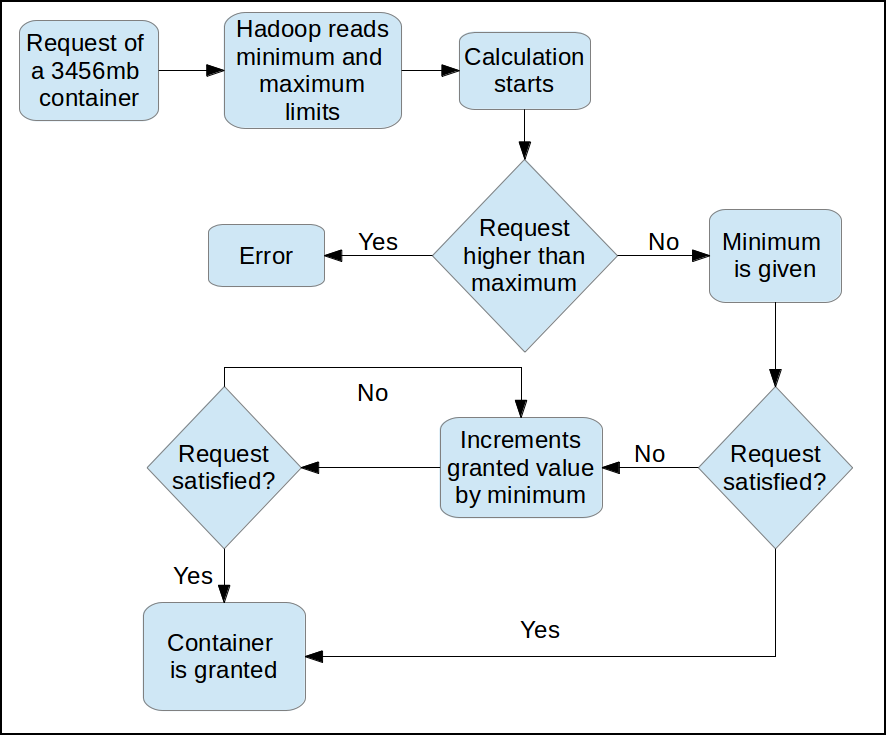
\includegraphics[width=15cm]{figuras/Figura19-allocflow2.png}
   \caption{Flow of operations for resource granting}
   \label{fig:fluxoAllocation2}
\end{figure}

The step by step calculation on scenario four will be demonstrated. Assuming M is the memory granted, or in the process of calculation, for the map request and R for the reduce. The calculation happens as follows:

Firstly the M and R are set to the minimum memory allocation property, which is 512. Since 512 does not satisfy any of the requests the M and R values are then incremented by the minimum memory allocation, assuming the value of 1024. As 1024 still smaller than both requisitions, they are again incremented by 512 and the process goes on as following:

M: 512, 1024, 1536, 2048, 2560, 3072, 3584.

R: 512, 1024, 1536, 2048, 2560, 3072, 3584, 4096.

Note that in both cases the value granted was the smallest multiple of minimum memory allocation (512) greater than or equal to the request (3456 and 3712).

%-------------------------------------------------------------------

\section{Context-aware scheduling}
Knowing that the scheduling task is closely related to the resources availability and, therefore, having a wrong information could ruin the performance of the algorithm, an opportunity for improvement was seen. After a quick study on the default schedulers, it was clear that CapacityScheduler already had the whole structure to support a better scheduling, as stated in the section \ref{sec:Hadoop Schedulers}. The flaw on CapacityScheduler wasn't really a scheduling flaw, but actually a wrong information received by the NodeManagers.

As stated numerous times in previous sections, Hadoop configuration is heavily dependent in XML files. While providing an easy way to configure a real cluster, sometimes it acts more as an obstacle than as a facilitator, the reason being that if one wants to change a parameter the whole service will have to be restarted. One huge restriction implied by XML files, is regarding the nodes capacity. In case one doesn't want to use Hadoop default configurations for node capacity, every node will have to have it's XML files edited. In a large heterogeneous cluster, modifying one file in each node will certainly be time consuming since each node will have a different configuration. 

One possible solution to this case, is to overwrite the value gotten from XML file on the code. At first glance this brings in more problems than solutions, because the administrator would have to chose a certain hard coded value that would fit best as an average among all nodes. However, as one looks closer into the proposal, there is an option that, although involving more coding, would solve this problem. 

It is clear that this solution requires the application to detect some context of the environment. The context, in this case, being the real information about node capacity. With this context at hands, it is a reasonable choice to make the scheduler context-aware. Therefore, improving the scheduling performance. As the section \ref{sec:ctx} implies, being context-aware requires the application to detect and adapt to changes in environment.

Regarding the detection of the node capacity, the chosen option was to integrate a collector into Hadoop, meaning that every node would be able to access it's true capacity. Thus, preventing the hard coding that was suggested.

Regarding the changes made once the context information was detected, the approach adopted was to scale the allocation limits together with the total cluster resource availability. This scaling meant that the containers would have more memory and cores at their disposal and, therefore, speculative task would hardly have to be launched. Also, by adapting to the cluster real resource, no resource would be wasted or left inactive while the scheduler is making tasks wait due to wrong information being received. Thus improving the cluster utilization.

\subsection{Collector description}
The collector of choice was PER-MARE's collector \cite{Collector}. This collector uses a standard java package in order to access the real node capacity, therefore, no additional libraries would be necessary.
 
Only four files were necessary, an interface, an abstract class and two classes. Due to it's design, it would be easy to integrate new collectors and improve the resources available for the scheduling process, providing data about the CPU load or disk usage for example.

The base of the collector is the interface Collector, which has two access methods and the collect method. 

The abstract class, called AbstractOSCollector, implements the interface and has some access methods of its own. The great usability comes from the usage of OperatingSystemMXBean, a public java interface that is used to access the operating system informations on which the Java virtual machine is running \cite{MXBean}.

The collector classes, called PhysicalMemoryColletor and TotalProcessorsCollector extends the AbstractOSCollector and have only constructor and collector method implemented.
%TODO trechos de c´odigo no appendix?

\subsection{Collector integration with Hadoop}
The collector would have to be placed on NodeManager (NM), since this is the service responsible for processing tasks. The collected capacity is then sent to the ResourceManager (RM) in the moment that each NM is registering with the RM. It is possible to view the whole process of data acquisition until CapacityScheduler add the node in the figure \ref{fig:collectorflow}.

\begin{figure}[!hbtn]
   \renewcommand{\figurename}{Figure}
   \centering
   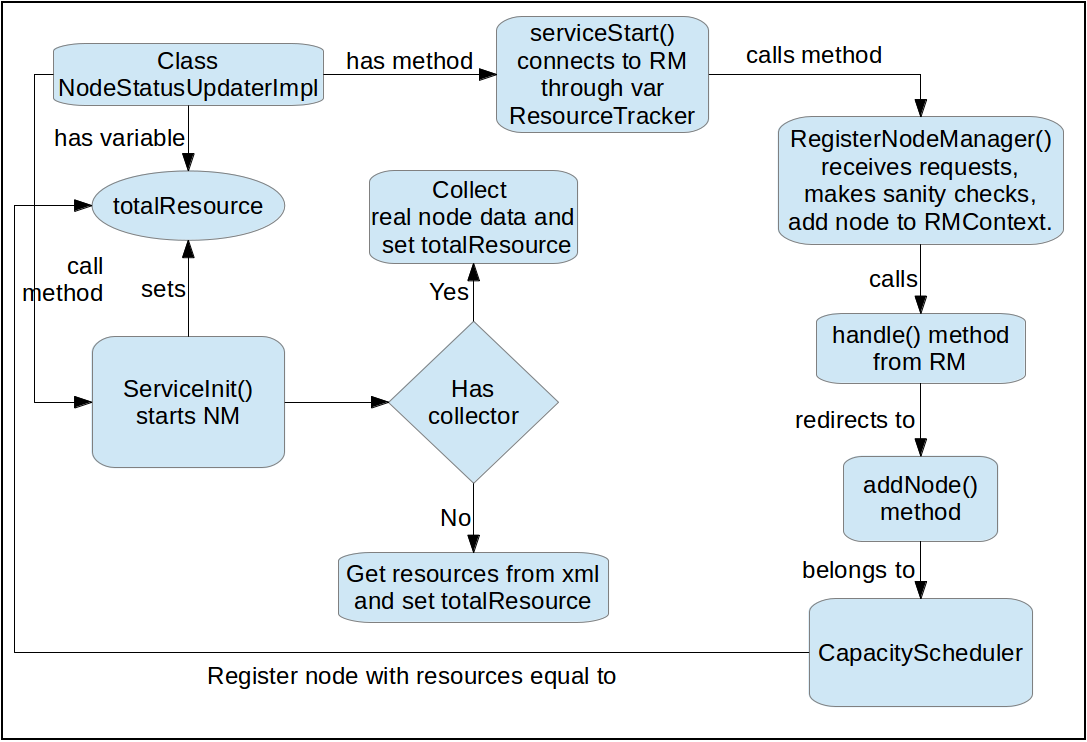
\includegraphics[width=15cm]{figuras/Figura20-collectorfig.png}
   \caption{Flow of operations for resource granting}
   \label{fig:collectorflow}
\end{figure}

After the collector integration, changing the scheduling behavior was possible due to the now available information about the real resources of a given node. Further information about the results gotten from the collector integration and modified scheduling can be found at the chapter \ref{chap:Experiments and Results}.
\chapter{Experimentos e Resultados}
\label{chap:ExpRes}
%-------------------------------------------------------------------
Este capítulo contém informações detalhadas sobre os experimentos realizados e os resultados obtidos. Embora o principal caso estudado foi o de degradação dos recursos em virtude de um compartilhamento dos nós, os experimentos realizados podem ser divididos em três categorias de acordo com seu objetivo. As três categorias são: (1) experimentos realizados em ambiente manipulado para verificação do desempenho da solução de forma simplificada; (2) experimentos realizados utilizando a implementação real para verificação do desempenho em ambiente controlado porém próximo à realidade; (3) experimentos em escala para visualização do desempenho com relação à escalabilidade da solução.

\section{Considerações Iniciais Sobre os Experimentos}
Em virtude de algumas informações sobre os experimentos serem comuns à todos eles, como os casos de teste e as aplicações utilizadas, esta Seção é destinada à apresentação destas informações. Além disso, a apresentação dos resultados utiliza diagramas de Gantt com uma estrutura modificada em relação à usualmente encontrada na literatura e será, também, explicada detalhadamente nesta Seção.

\subsection{Casos de teste}
\label{sec:casosteste}
A primeira informação relevante que refere-se à todos experimentos são os casos de teste. Todos os experimentos utilizam os mesmos casos de teste, possuindo apenas objetivos diferentes. Os casos de teste representam situações de compartilhamento, sendo que 2 casos utilizam a implementação padrão e 2 casos utilizam a solução proposta por este trabalho. Além disso, com a criação dos casos de teste buscou-se facilitar a comparação entre os resultados alcançados. A descrição dos casos de testes encontra-se a seguir.

\textbf{Caso Adaptativo com atualização antes (AdaptBef):} utiliza a implementação descrita no Capítulo \ref{cap:desen} e representa a situação decorrente do compartilhamento dos nós do \textit{cluster} com outros usuários. Este caso representa a situação de quando o início do compartilhamento ocorre \textbf{antes} da coleta e transmissão de dados, a qual ocorre também \textbf{antes} do lançamento de uma aplicação \textit{MapReduce}. Em ordem cronológica, primeiramente outro usuário inicia a utilização do \textit{cluster}, então a coleta e transmissão de dados ocorre, e finalmente uma aplicação Hadoop é lançada. O resultado desta sequência de eventos é que quando a nova aplicação \textit{MapReduce} for submetida ao \textit{cluster}, este já estará com os dados atualizados. Para representar a situação onde apenas alguns nós são utilizados compartilhadamente, optou-se por deixar alguns nós inalterados e outros com redução de recursos. Nos experimentos de 4 escravos, 2 nós tiveram 6 \textit{cores} e 6 Gb de RAM reduzidos através de um código C, restando 2Gb e 2 \textit{cores} para o SO e Hadoop. Em notação percentual, os recursos informados são de 62,5\% e os recursos disponíveis são de 62,5\% durante toda aplicação.

\textbf{Caso Adaptativo com atualização durante (AdaptDur):} representa uma extensão do Caso AdaptBef (também utilizando a implementação do Capítulo \ref{cap:desen}) na qual o início do compartilhamento ocorre \textbf{antes} da coleta e transmissão dos dados, porém \textbf{após} a submissão de uma aplicação \textit{MapReduce}. Em ordem cronológica, ocorre o lançamento de uma aplicação \textit{MapReduce}, então quando esta aplicação já está em execução o compartilhamento tem início e finalmente a coleta e transmissão de dados é feita. O resultado desta sequência de eventos é que a aplicação será lançada numa situação onde o \textit{cluster} possui a informação errada (Caso DefSha) e terá de se adaptar à nova configuração dos recursos (Caso AdaptBef) durante a execução. Utiliza o mesmo método de redução de recursos que o caso AdaptBef. Em notação percentual, os recursos informados no início da aplicação são de 100\%, enquanto os recursos disponíveis são de 62,5\%. Após a coleta e transmissão de dados os recursos informados também passam a ser 62,5\%.

\textbf{Caso \textit{Default} Dedicado (DefDed):} utiliza a versão sem alterações do Hadoop e representa uma situação sem compartilhamento, onde o usuário possui acesso à todos os recursos do \textit{cluster} em qualquer momento. Isto implica que os recursos informados ao escalonador corresponderão aos recursos disponíveis para o Hadoop durante toda execução. Consideram-se recursos informados como os dados que o escalonador utiliza para realizar suas políticas de escalonamento, enquanto, recursos disponíveis são aqueles que estão livres e/ou sendo utilizados pelo próprio Hadoop. Utilizando uma notação percentual, os recursos informados são de 100\% e os recursos disponíveis são de 100\% durante toda execução.

\textbf{Caso \textit{Default} Compartilhado (DefSha):} utiliza a versão sem alterações do Hadoop e representa a situação decorrente do compartilhamento dos nós do \textit{cluster} com outros usuários. Como consequência do compartilhamento, é possível que em, algum momento, ocorra uma inconsistência entre a quantidade de recursos informada e disponível. Este caso aplica o comportamento padrão do Hadoop, no qual os recursos são informados por meio de arquivos XML \textbf{somente} na inicialização do serviço e nunca são atualizados. Utiliza o mesmo método de redução de recursos que o caso AdaptBef. No contexto do cluster, os recursos informados são de 100\% enquanto os disponíveis são de 62,5\%.

\subsection{Aplicações de teste}
\label{sec:aplicacoes}
Além dos casos de teste, outra característica importante e comum à todos experimentos são as aplicações. Embora aplicações de \textit{Benchmarks} geralmente possuem dependência de memória, outros fatores como a utilização de CPU e E/S podem influenciar no desempenho. Na busca de indícios de que a solução apresenta ganhos quando utilizada com aplicações de diferentes características, decidiu-se pela utilização de 3 aplicações de \textit{benchmark}, cada uma com diferentes requisições de memória, CPU e E/S. As aplicações são as seguintes:

\begin{itemize}
	\item TeraSort: o objetivo do TeraSort \citet{TeraSort2008} é ordenar um conjunto de dados o mais rápido possível. Este \textit{benchmark} de ordenação estressa tanto a memória como o CPU em virtude das comparações e armazenamento temporário;
	\item WordCount: o \textit{benchmark} WordCount é um exemplo básico de \textit{MapReduce}. Seu objetivo é contar o número de ocorrências de cada palavra de um texto. Como a utilização de memória e E/S é limitada nesta aplicação (tanto a etapa de processamento quanto a saída da aplicação possuem estruturas pequenas em comparação ao arquivo de entrada), o desempenho desta aplicação é determinado pelo CPU;
	\item TestDFSIO: o \textit{benchmark} TestDFSIO é um teste de leitura e escrita para o HDFS. Este \textit{benchmark} é útil para estressar o HDFS, descobrir \textit{bottlenecks} na rede, SO e configuração do Hadoop. O objetivo é prover uma mensuração de quão rápido o \textit{cluster} é em termos de E/S. Tanto a memória quanto o CPU são pouco utilizados.
\end{itemize}

Optou-se pela utilização das aplicações implementadas no \textit{HiBench} \cite{HiBench}, um conjunto de \textit{benchmarks} para \textit{clusters} Hadoop que foi utilizado nos trabalhos \cite{HBA} \cite{HBB} \cite{HBC}. O tamanho de entrada utilizado para cada aplicação nos testes com 4 escravos foi: um conjunto de dados de 15 Gb para o Terasort, 90 arquivos de 250 Mb para o TestDFSIO e um arquivo de 10 Gb para o WordCount. Além disso, cada experimento utilizou a mesma entrada para a execução dos 4 casos propostos.

\subsection{Configurações de Hardware e Software}
O experimento foi realizado no \textit{cluster} genepi do Grid'5000. A configuração do \textit{cluster} utilizado na maior parte dos experimentos foi a de 1 mestre e 4 escravos, sendo que cada um destes nós possuem a seguinte configuração: 2 CPUs Intel(R) Xeon(R) E5420 2.5GHz (totalizando 8 cores por nó) e 8 Gb RAM. Todos os nós do experimento possuíam o sistema operacional Ubuntu x64-12.04, com a JDK 1.8 instalada e a versão 2.6.0 do Hadoop configurada. Todas as informações foram obtidas através do sistema de \textit{logs} do Hadoop.

\subsection{Apresentação dos resultados}
\label{sec:apresentacao}
Ainda ligado aos experimentos porém com relação aos resultados, os diagramas de Gantt apresentados neste trabalho são modificados para inclusão de mais informações. A apresentação dos diagramas está agrupada por aplicação, sendo que e cada aplicação possui, geralmente, 4 diagramas. Cada um dos diagramas de uma aplicação corresponde a um caso de teste e todos os diagramas de uma aplicação utilizam a mesma escala de tempo.

Cada diagrama possui 2 ou mais linhas, sendo que cada linha representa  um recurso (nó do \textit{cluster}). Estas linhas de recurso possuem diversos separadores verticais (formando diversos segmentos), os quais indicam que ao menos um \textit{container} iniciou/terminou sua execução. Cada segmento apresenta diferentes alturas e tons de cores, os quais são utilizados para representar a carga de \textit{containers Map} do nó. Quanto mais escuro for o tom de um segmento, mais \textit{containers} ele possui em execução; o mesmo aplica-se para a altura do segmento, quanto mais alto mais \textit{containers Map} em execução.

Embora as análises foram feitas principalmente com os \textit{containers} Map, os \textit{containers} de Reduce e do Application Master consomem recursos do \textit{cluster} e devem ser apresentados para uma representação fiel da situação real. Por este motivo, o \textit{container} Application Master é representado na cor azul, os \textit{containers} de Reduce são representados pela cor verde e os \textit{containers} Map são representados em escalas de cinza, sendo branco indicando 0 \textit{containers} e preto indicando o máximo de \textit{containers} em execução em algum momento naquele experimento. Para referência, diagramas da Seção \ref{sec:expCont} possuem máximo de 16, enquanto diagramas das demais Seções possuem máximo de 8.

\section{Experimento controlado}
\label{sec:expCont}
Este experimento foi realizado com objetivo de obter indícios de que a solução poderia contribuir para uma melhora no desempenho do processo de escalonamento quando o Hadoop é utilizado num ambiente onde exista degradação de recursos em virtude de compartilhamento. O experimento simplifica a solução para facilitar a obtenção dos dados em menor tempo. A situação que desejou-se expressar com o experimento é aquela que ocorre quando os nós do \textit{cluster} começam a ser utilizados por outros usuários antes/durante a aplicação \textit{MapReduce}.

\subsection{Procedimentos}
Para que o experimento fosse totalmente controlado, decidiu-se utilizar a manipulação de informações e exclusão de nós para representar o compartilhamento. Na situação real (ver Seção \ref{sec:expReal}) o \textit{cluster} teria 4 escravos e ficaria com uma configuração onde metade dos seus recursos já estariam sendo utilizados por outra aplicação. Por exemplo, outra aplicação utilizaria 4 cores e 4 Gb de memória em cada nó. Para representar esta situação de maneira simples e rápida, o experimento foi realizado com apenas 2 nós (diminuindo os recursos disponíveis pela metade) que tiveram a informação da quantidade de recursos dobrada. Como resultado, o escalonador recebe informação de que os recursos disponíveis são de 16 cores e 16 Gb de memória em cada nó quando na verdade são de apenas 8 cores e 8 Gb. 

Foram realizados experimentos com as 3 aplicações para que as diferenças de comportamento entre elas já pudessem ser estudadas num cenário de sobrecarga de memória e processamento.

\subsection{Resultados e Interpretações}
Os resultados dos experimentos com as aplicações TeraSort, TestDFSIO e WordCount podem ser visualizados nas Tabelas \ref{tab:exp1TS}, \ref{tab:exp1IO} e \ref{tab:exp1WC} e nas Figuras \ref{fig:exp1TS}, \ref{fig:exp1IO} e \ref{fig:exp1WC}, respectivamente.

\begin{table}[!ht]
	\caption{Resumo dos resultados do TeraSort controlado em segundos.} \label{tab:exp1TS}
	\begin{tabular*}{\hsize}{lllll}
		\textbf{Caso} & \textbf{DefDed} & \textbf{DefSha} & \textbf{AdaptBef} & \textbf{AdaptDur}\\
		\hline
		Tempo Total de Map ({\it{s}}) & 149 & 788 & 348 & 477 \\
		Tempo Médio de Map ({\it{s}}) & 39.47 & 222.97 & 38.38 & 68.42 \\
		\# Tarefas Map & 76 & 76 & 76 & 76 \\
		\# Tarefas Especulativas & 2 & 1 & 3 & 1 \\
	\end{tabular*}
\end{table}

\begin{table}[!ht]
	\caption{Resumo dos resultados do TestDFSIO controlado em segundos.} \label{tab:exp1IO}
	\begin{tabular*}{\hsize}{lllll}
		\textbf{Caso} & \textbf{DefDed} & \textbf{DefSha} & \textbf{AdaptBef} & \textbf{AdaptDur}\\
		\hline
		Tempo Total de Map ({\it{s}}) & 139 & 444 & 239 & 364 \\
		Tempo Médio de Map ({\it{s}}) & 38.95 & 85.01 & 32.20 & 81.62 \\
		\# Tarefas Map & 90 & 90 & 90 & 90 \\
		\# Tarefas Especulativas & 0 & 9 & 0 & 1 \\
	\end{tabular*}
\end{table}


\begin{table}[!ht]
	\caption{Resumo dos resultados do WordCount controlado em segundos.} \label{tab:exp1WC}
	\begin{tabular*}{\hsize}{lllll}
		\textbf{Caso} & \textbf{DefDed} & \textbf{DefSha} & \textbf{AdaptBef} & \textbf{AdaptDur}\\
		\hline
		Tempo Total de Map ({\it{s}}) & 155 & 1009 & 309 & 805 \\
		Tempo Médio de Map ({\it{s}}) & 43.76 & 208.39 & 41.73 & 175.80 \\
		\# Tarefas Map & 90 & 90 & 90 & 90 \\
		\# Tarefas Especulativas & 1 & 15 & 1 & 10 \\
	\end{tabular*}
\end{table}

\begin{figure}[!ht]
	\centering
	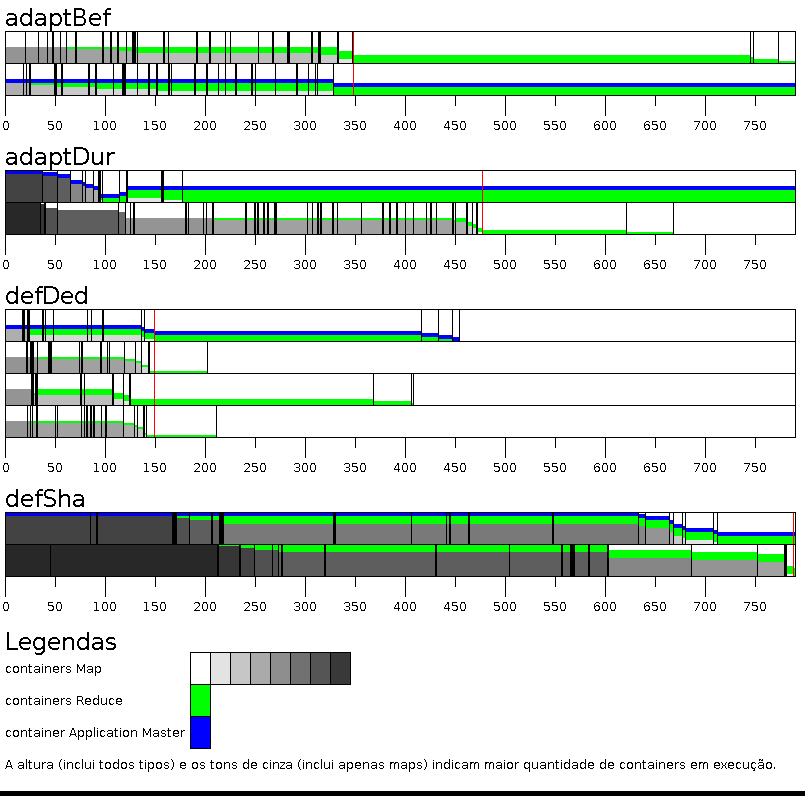
\includegraphics[height=15cm]{figuras/TS-simul.png}
	\caption{Diagrama de Gantt para os experimentos controlados com TeraSort}
	\label{fig:exp1TS}
\end{figure}

\begin{figure}[!ht]
	\centering
	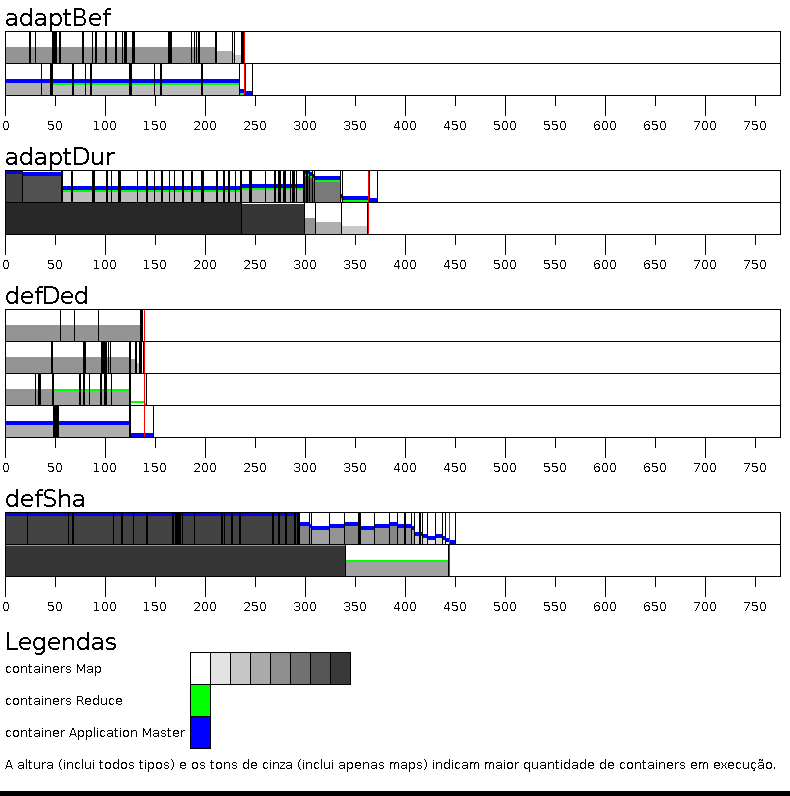
\includegraphics[height=15cm]{figuras/DFS-simul.png} 
	\caption{Diagrama de Gantt para os experimentos controlados com TestDFSIO}
	\label{fig:exp1IO}
\end{figure}

\begin{figure}[!ht]
	\centering
	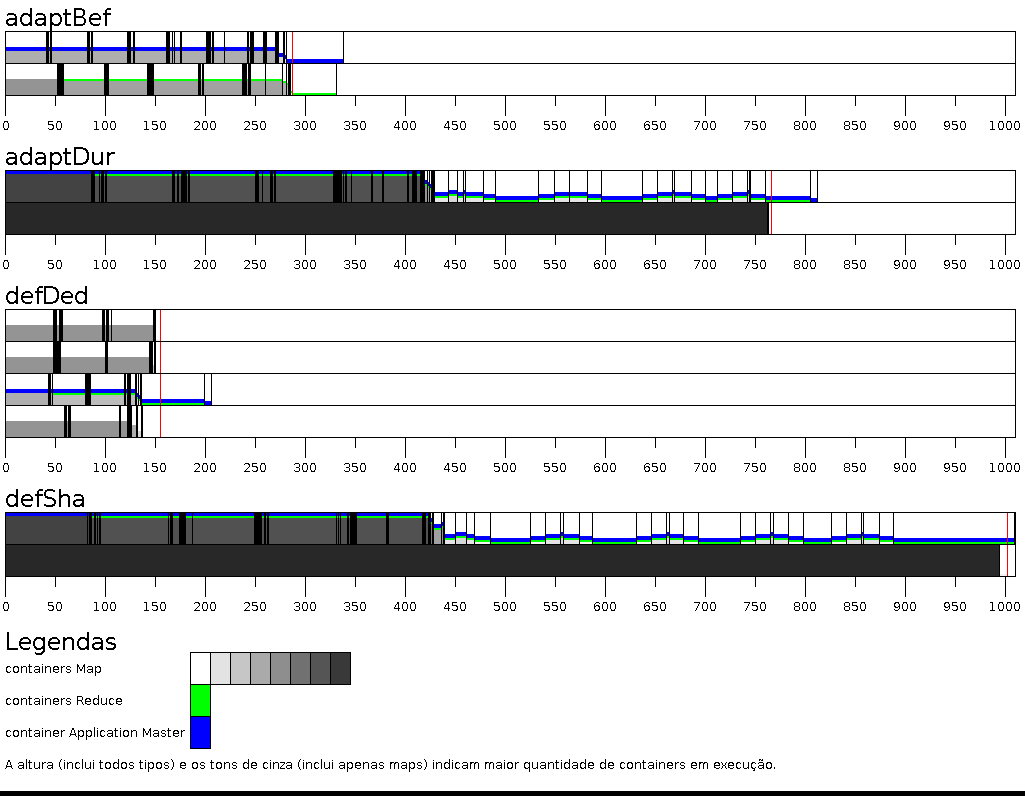
\includegraphics[height=15cm]{figuras/WC-simul.png}
	\caption{Diagrama de Gantt para os experimentos controlados com WordCount}
	\label{fig:exp1WC}
\end{figure}

Analisando as tabelas, é possível identificar alguns padrões. Todos experimentos apresentam um comportamento similar com relação ao tempo total dos \textit{containers Map}: DefDed foi o mais rápido, seguido pelos casos AdaptBef, AdaptDur e finalmente DefSha. Ainda, os casos DefDed e AdaptBef possuem os menores tempos médios de \textit{Map} e estes são muito semelhantes não importando a aplicação analizada. Este comportamento é devido à não sobrecarga dos nós, uma vez que o escalonador possuia os dados corretos com relação aos recursos dos nós durante todo experimento.
Os diagramas de Gantt também apresentam esta informação uma vez que os experimentos DefDed e AdaptBef possuem tons mais claros e alturas menores do que os demais no início da aplicação, o que significa que há menos \textit{containers} em execução. É possível notar também que o caso AdaptBef leva, em geral, o dobro do tempo do caso DefDed para terminar a etapa de Map. Este resultado é esperado, uma vez que neste experimento o caso DefDed possui o dobro de recursos disponíveis se comparado com o caso AdaptBef. 

Outra observação interessante tem relação com a análise das tarefas especulativas iniciadas em cada aplicação. A aplicação TeraSort possui um número reduzido de tarefas iniciadas e este número é similar em todos os casos. Já o TestDFSIO e o WordCount apresentam um alto número de tarefas especulativas nos casos em que o sistema está sobrecarregado em algum momento (DefSha e AdaptDur). Este comportamento pode ser explicado sob a análise dos fatores que determinam o lançamento ou não de uma tarefa especulativa. Sabe-se que uma tarefa especulativa é iniciada com base numa avaliação de progresso da tarefa, onde uma tarefa atrasada em relação às demais está possivelmente apresentando falhas. No caso do TeraSort, onde as tarefas demandam de maneira uniforme os recursos de memória, CPU e E/S, o tempo de execução está menos sujeito à redução de um recurso específico. Enquanto o TestDFSIO e o WordCount, demandam recursos mais específicos e, portanto, são mais sensíveis à sobrecarga destes recursos. Em todas as aplicações, a utilização de sensibilidade ao contexto como meio de melhorar a adaptabilidade no caso AdaptDur ajuda a reduzir o número de tarefas especulativas quando comparado com o caso DefSha que não apresenta nenhuma capacidade de adaptação à estes ambientes.

Com relação ao fluxo de execução, como ilustrado nos diagramas, é possível notar que os casos DefSha e AdaptDur possuem tons mais escuros no início, o que significa que cada nó está com 16 \textit{containers} em execução (o dobro da capacidade real do nó). Ainda, os primeiros \textit{containers} a terminar nos casos DefDed e AdaptBef levam entre 20 e 50 segundos (conforme linha vertical de segmento), enquanto nos casos DefSha (e em menor grau AdaptDur) os primeiros \textit{containers} levam 70 segundos ou mais para terminar, evidenciando a sobrecarga dos nós. As excessões à esta afirmação são os casos DefSha e AdaptDur do TestDFSIO, nos quais os primeiros \textit{containers} a terem o processamento concluído levam aproximadamente 25 segundos para tal. Através de uma análise mais profunda, é possível notar que todos os casos do experimento TestDFSIO possuem ao menos um seguimento próximo à marca dos 25 segundos, o que significa que uma das tarefas deste conjunto de entrada foi processada rapidamente em todos os casos, e não foi afetada pela sobrecarga dos nós nos casos DefSha e AdaptDur.

Embora os casos DefSha e AdaptDur possuam as mesmas condições iniciais (recursos disponíveis de 50\% e recursos informados de 100\%), o caso AdaptDur necessita de menos tempo para concluir o processamento da aplicação em todas as aplicações. O caso AdaptDur possui uma melhora de 20\% a 40\% no tempo de execução quando comparado com o caso DefSha. A razão para este comportamento é a capacidade de adaptação inserida ao Hadoop, a qual permite que os Node Managers coletem a informação correta e à transmitam para o escalonador, que irá reorganizar a distribuição de tarefas à medida que as tarefas em execução são concluídas. Este comportamento é mais fácil de ser observado nos diagramas das aplicações TeraSort e TestDFSIO. É possível notar também que todos o casos AdaptDur possuem alta concentração de containers no início da aplicação mas essa concentração diminui ao longo da execução, enquanto os casos DefSha mantém a alta concentração até os últimos momentos da execução devido à ausencia de adaptabilidade. Embora o escalonador não preempte \textit{containers} em excesso, é possível observar uma melhora de aproximadamente 40\% no TeraSort e 20\% no TestDFSIO e WordCount apenas pela inibição do lançamento de novos \textit{containers} enquanto o nó está sobrecarregado.


%Although other specificities about the characteris-
%tics of the proposed jobs can be discussed, scenarios C
%and D show that regular context updates contribute to
%reduce the execution time on a dynamic Hadoop clus-
%ter. We demonstrated that even when starting with the
%same circumstances of the worst case (Scenario B), up-
%dating the information helps the scheduler to minimize
%the execution time. Our solution contributes therefore
%to both provide correct information before the execu-
%tion starts (Scenario C) and to adapt the execution to
%resources changes (Scenario D).
%CONCLUSÂO

\section{Experimento real}
\label{sec:expReal}
Este experimento foi realizado com objetivo de obter indícios de que a solução poderia contribuir para uma melhora no desempenho do processo de escalonamento quando o Hadoop é utilizado num ambiente onde exista degradação de recursos em virtude de compartilhamento. O experimento utiliza a solução descrita no Capítulo \ref{cap:desen}. A situação expressada com este experimento é de quando os nós do \textit{cluster} começam a ser utilizados por outros usuários antes/durante a aplicação \textit{MapReduce}.

\subsection{Procedimentos}
Diferentemente do experimento anterior, neste experimento buscou-se o comportamento da solução em um ambiente realmente compartilhado. O \textit{cluster} possui 4 escravos e alguns escravos terão, em algum momento, seus recursos disponíveis reduzidos devido ao compartilhamento, ou seja, outra aplicação irá utilizar 6 cores e 6 Gb de memória em 2 dos 4 nós escravos. Para alcançar esta situação foi implementada uma aplicação em C, na qual a quantidade desejada de \textit{threads} é inicializada e cada uma delas utiliza 1 core e 1 Gb de memória. O experimento foi realizado com as 3 aplicações para observações de possíveis alterações no comportamento com relação ao experimento inicial.

\subsection{Resultados e Interpretações}
Os resultados dos experimentos com as aplicações TeraSort, TestDFSIO e WordCount podem ser visualizados nas Tabelas \ref{tab:exp2TS}, \ref{tab:exp2IO} e \ref{tab:exp2WC} e nas Figuras \ref{fig:exp2TS}, \ref{fig:exp2IO} e \ref{fig:exp2WC}, respectivamente.

\begin{table}[!ht]
	\caption{Resumo dos resultados do TeraSort real em segundos.} \label{tab:exp2TS}
	\begin{tabular*}{\hsize}{lllll}
		\textbf{Caso} & \textbf{DefDed} & \textbf{DefSha} & \textbf{AdaptBef} & \textbf{AdaptDur}\\
		\hline
		Tempo Total de Map ({\it{s}}) & 281 & 1372 & 740 & 888 \\
		Tempo Médio de Map ({\it{s}}) & 38.50 & 198.86 & 39.58 & 62.82 \\
		\# Tarefas Map & 112 & 112 & 112 & 112 \\
		\# Tarefas Especulativas & 1 & 14 & 0 & 2 \\
	\end{tabular*}
\end{table}

\begin{table}[!ht]
	\caption{Resumo dos resultados do TestDFSIO real em segundos.} \label{tab:exp2IO}
	\begin{tabular*}{\hsize}{lllll}
		\textbf{Caso} & \textbf{DefDed} & \textbf{DefSha} & \textbf{AdaptBef} & \textbf{AdaptDur}\\
		\hline
		Tempo Total de Map ({\it{s}}) & 194 & 674 & 264 & 431 \\
		Tempo Médio de Map ({\it{s}}) & 31.24 & 162.47 & 38.56 &  65.24 \\
		\# Tarefas Map & 90 & 90 & 90 & 90 \\
		\# Tarefas Especulativas & 2 & 16 & 0 & 8 \\
	\end{tabular*}
\end{table}


\begin{table}[!ht]
	\caption{Resumo dos resultados do WordCount real em segundos.} \label{tab:exp2WC}
	\begin{tabular*}{\hsize}{lllll}
		\textbf{Caso} & \textbf{DefDed} & \textbf{DefSha} & \textbf{AdaptBef} & \textbf{AdaptDur}\\
		\hline
		Tempo Total de Map ({\it{s}}) & 153 & 533 & 361 & 396 \\
		Tempo Médio de Map ({\it{s}}) & 34.85 & 105.27 & 37.79 & 57.76 \\
		\# Tarefas Map & 90 & 90 & 90 & 90 \\
		\# Tarefas Especulativas & 1 & 14 & 1 & 2 \\
	\end{tabular*}
\end{table}

\begin{figure}[!ht]
	\centering
	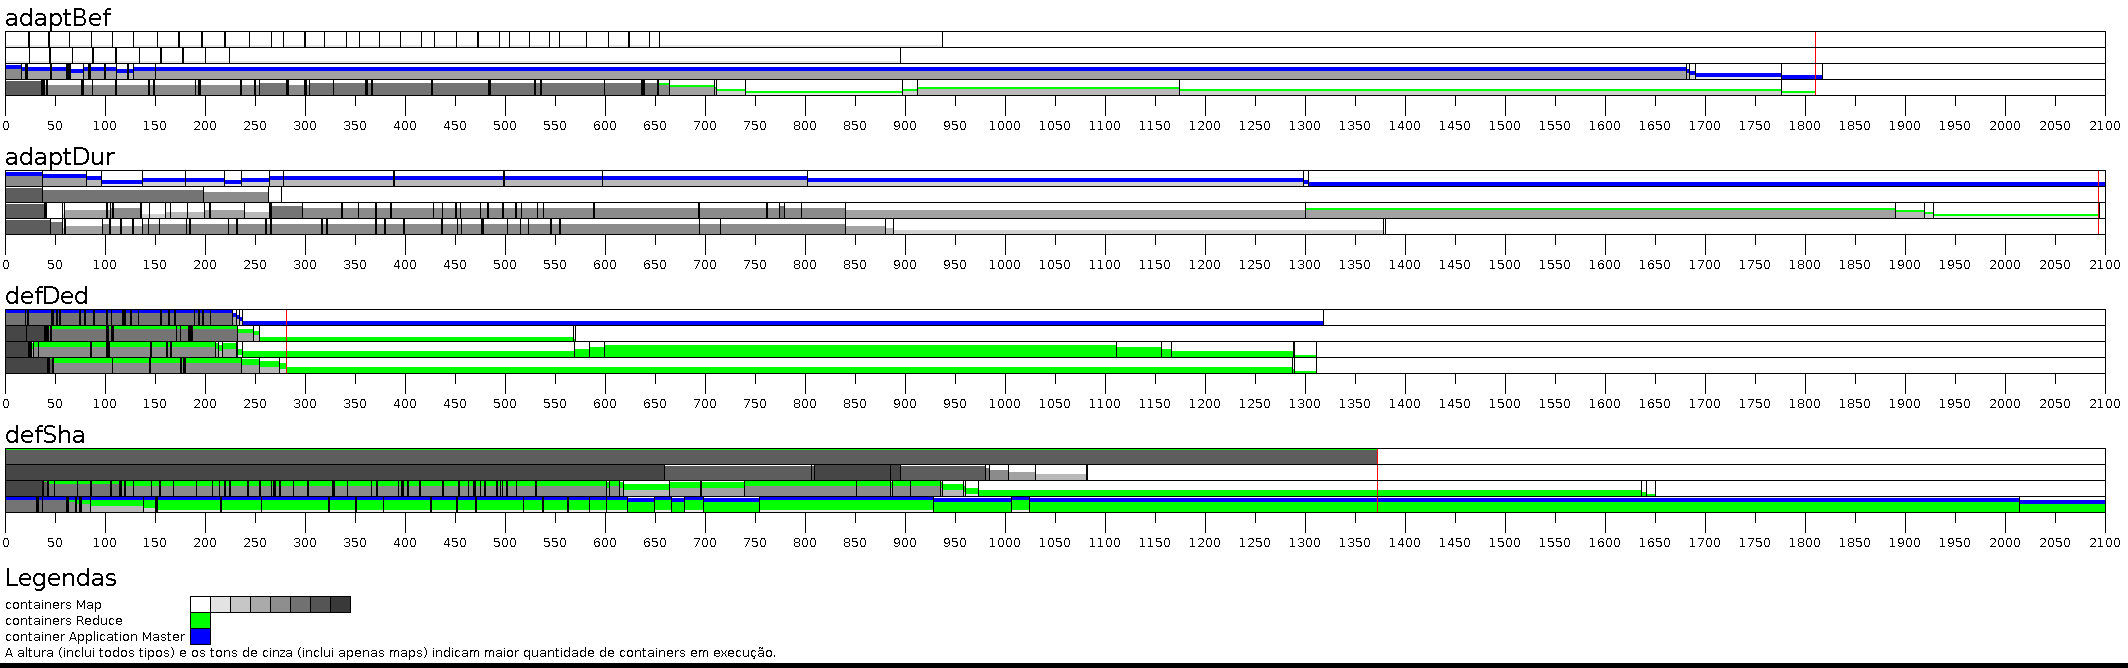
\includegraphics[width=1\textwidth]{figuras/TS-real.png}
	\caption{Diagrama de Gantt para os experimentos reais com TeraSort}
	\label{fig:exp2TS}
\end{figure}

\begin{figure}[!ht]
	\centering
	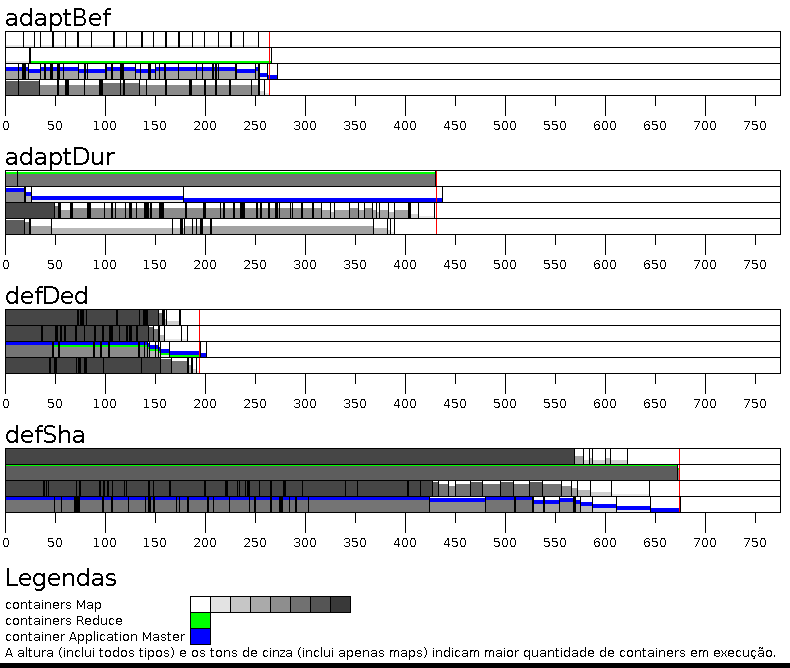
\includegraphics[height=15cm]{figuras/DFS-real.png}
	\caption{Diagrama de Gantt para os experimentos reais com TestDFSIO}
	\label{fig:exp2IO}
\end{figure}

\begin{figure}[!ht]
	\centering
	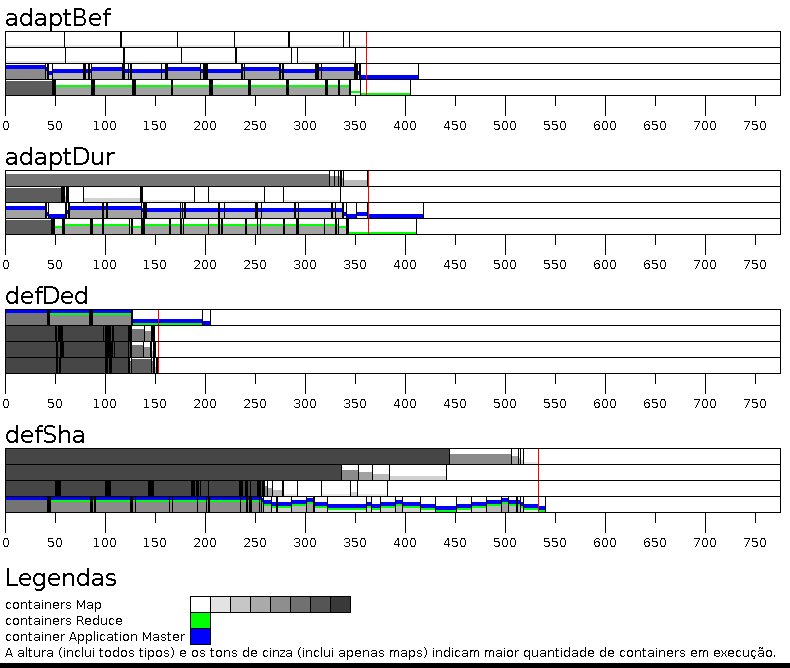
\includegraphics[height=15cm]{figuras/WC-real.png}
	\caption{Diagrama de Gantt para os experimentos reais com WordCount}
	\label{fig:exp2WC}
\end{figure}

Através da análise das tabelas e dos diagramas, nota-se que muitos padrões foram mantidos apesar da alteração de procedimento nos experimentos. Primeiramente, é importante notar que nas aplicações anteriores a sobrecarga dos nós era de 100\%, uma vez que o Hadoop estava tentando utilizar o dobro da capacidade. Na execução das aplicações deste experimento a sobrecarga é levemente menor, pois a informação passada ao Hadoop nos casos default não é alterada. A sobrecarga nestes experimentos é de aproximadamente 6 Gb de RAM e 6 cores, fazendo com que o nó, nos piores casos, tenha uma demanda de aproximadamente 14 Gb e 14 cores (sem considerar recursos requisitados pelo sistema operacional e serviços do Hadoop) alocada aos seus 8 Gb e 8 cores.

Novamente, todas aplicações apresentam um comportamento similar com relação ao tempo total dos \textit{containers Map} e tempo médio destes: DefDed apresentou o menor tempo total e médio dos \textit{containers Map}, seguido pelos casos AdaptBef, AdaptDur e finalmente DefSha. Também seguindo o padrão do experimento anterior, os tempos médio de Map nos casos DefDed e AdaptBef são muito semelhantes não importando a aplicação analizada. Embora alguns padrões foram mantidos, a proporção de tempo entre os casos DefDed e AdaptBef não apresenta uma relação tão constante quanto no experimento anterior e algumas particularidades podem ser observadas nos diagramas. Ainda assim, estes dados iniciais sugerem que uma sobrecarga de alguns nós, mesmo em menor intensidade se comparado ao experimento anterior, deteriora significativamente o desempenho da aplicação.

Com relação às tarefas especulativas, nota-se que neste experimento o caso DefSha apresentou um número alto de tarefas especulativas nas 3 aplicações, enquanto os demais casos mantiveram valores baixos salvo o caso AdaptDur na aplicação TestDFSIO. Os resultados deste experimento sugerem que embora a sobrecarga, com relação à demanda total, tenha sido menor, os efeitos provocados por ela foram mais visíveis, pois os casos onde a sobrecarga esteve presente durante toda aplicação apresentam um número elevado de tarefas especulativas.

Antes de realizar a análise dos diagramas deste experimento é necessário salientar uma característica importante, todos os diagramas a gerados para este experimento possuem no máximo 8 \textit{containers} em execução, enquanto no experimento anterior este valor era de 16. Além disso, os diagramas possuem características que permitem uma visualização das tarefas que originam tarefas especulativas e da reação à mudança de recursos nos nós. 

Nas 3 aplicações o caso AdaptBef pode, em um primeiro momento, aparentar estar com 2 nós sem utilização, porém este comportamento é exatamente o esperado dos nós. O caso de teste é criado de forma que quando outro usuário utiliza o \textit{cluster}, ele demanda 6 Gb e 6 cores de 50\% dos nós, deixando apenas 2 Gb e 2 cores disponíveis para o sistema operacional e o Hadoop. Retirando os recursos do sistema operacional e dos serviços do Hadoop restam pouco mais de 1 Gb e 1 core livres, com os quais o Hadoop pode lançar apenas 1 \textit{container} nos nós compartilhados. Com apenas 1 \textit{container} em execução, o diagrama apresenta uma cor próxima do branco e a altura de somente 1/8 da linha, tornando a visualização de \textit{containers} Map difícil. No caso de um \textit{container} Reduce em execução, como no diagrama AdaptBef do TestDFSIO, a cor verde facilita a visualização.

Nos diagramas gerados para os casos AdaptDur da aplicação TestDFSIO é possível notar que um dos nós termina uma carga de 6 a 7 containers simultaneamente e que logo após isso a aplicação toda é concluída. Uma rápida consulta à tabela fornece a informação de que nessa aplicação o número de tarefas especulativas no caso AdaptDur foi o mais elevado das 3 aplicações. Além disso, a análise dos logs mostra que a última tarefa especulativa termina 2 segundos antes do término de todos \textit{containers} do primeiro nó. Estas duas observações sugerem que a sobrecarga do nó compartilhado impediu o término gradual dos \textit{containers} lentos à medida que suas cópias especulativas finalizavam a execução. Este mesmo comportamento pode ser observado no caso DefSha.

Apesar das condições e mecanismos de compartilhamento/atualização implementados nos testes reais serem diferentes daqueles implementados nos testes controlados, os diagramas deste experimento também apresentam reação ao início do compartilhamento. É possível notar uma redução gradual dos recursos nos dois primeiros nós na maioria dos casos AdaptDur. Além disso, é possível notar que a linha nunca fica completamente colorida nos casos AdaptBef e AdaptDur, indicando que o coletor detectou os recursos utilizados pelo sistema operacional e excluiu os mesmos do \textit{pool} de recursos do Hadoop.

Mais uma vez as execuções do caso AdaptDur apresentam uma melhora entre 36\% e 24\% no tempo total de Map comparado com o caso DefSha, mostrando que a detecção da sobrecarga no nó e a adaptação do processo de escalonamento para eventualmente eliminar a sobrecarga melhora o desempenho da aplicação. Ainda com relação ao tempo total de Map, nota-se que quanto maior a duração da aplicação maior é o ganho de desempenho pela utilização do escalonamento adaptativo. Os resultados também indicam que a adaptação do escalonamento em função da sobrecarga diminui a quantidade de tarefas especulativas e o tempo médio que as tarefas Map levam para concluir a execução. 


\section{Experimento de escala}
Uma vez que os experimentos anteriores já responderam algumas questões importantes sobre a viabilidade da solução implementada, este experimento foi realizado com objetivo de analisar se as melhorias no escalonamento são mantidas quando o Hadoop é utilizado em um ambiente ou com uma entrada de dados maior. O experimento utiliza a solução descrita no Capítulo \ref{cap:desen}. A situação expressada com este experimento é de quando os nós do \textit{cluster} começam a ser utilizados por outros usuários antes/durante a aplicação \textit{MapReduce}.

\subsection{Procedimentos}
Neste experimento buscou-se analisar o comportamento da solução em um ambiente compartilhado de maior escala que nos experimentos anteriores. Foram feitos 2 experimentos distintos, um com escala de aplicação outro com escala de ambiente. Para a escala de aplicação a única diferença das configurações foi o tamanho da entrada, sendo utilizada uma entrada de 32 Gb para o TeraSort. Para a escala de ambiente, utilizou-se um \textit{cluster} com 10 escravos e entrada de 40 Gb, sendo que a proporção de recursos reduzidos/livres continuou a mesma. 

\subsection{Resultados e Interpretações}
Os resultados dos experimentos em escala (de entrada e de ambiente) com a aplicação TeraSort podem ser visualizados nas Tabelas \ref{tab:exp3TS} e \ref{tab:exp31TS} e nas Figuras \ref{fig:exp3TS} e \ref{fig:exp31TS}, respectivamente.

\begin{table}[!ht]
	\caption{Resumo dos resultados do TeraSort em escala (tamanho da entrada) em segundos.} \label{tab:exp3TS}
	\begin{tabular*}{\hsize}{l|llll}
		\textbf{Caso} & \textbf{DefDed} & \textbf{DefSha} & \textbf{AdaptBef} & \textbf{AdaptDur}\\
		\hline
		Tempo Total de Map ({\it{s}}) & 1357 & 4627 & 2060 & 2184 \\
		Tempo Médio de Map ({\it{s}}) & 43.39 & 299.70 & 45.36 & 65.00 \\
		\# Tarefas Map & 240 & 240 & 240 & 240 \\
		\# Tarefas Especulativas & 1 & 27 & 0 & 5 \\
	\end{tabular*}
\end{table}
%
%


\begin{table}[!ht]
	\caption{Resumo dos resultados do TeraSort em escala (tamanho do ambiente) em segundos.} \label{tab:exp31TS}
	\begin{tabular*}{\hsize}{l|llll}
		\textbf{Caso} & \textbf{DefDed} & \textbf{DefSha} & \textbf{AdaptBef} & \textbf{AdaptDur}\\
		\hline
		Tempo Total de Map ({\it{s}}) & 273 & 2138 & 743 & 1421 \\
		Tempo Médio de Map ({\it{s}}) & 55.69 & 322.66 & 51.49 & 85.35 \\
		\# Tarefas Map & 298 & 298 & 298 & 298 \\
		\# Tarefas Especulativas & 2 & 26 & 1 & 1 \\
	\end{tabular*}
\end{table}
%
%

\begin{sidewaysfigure}
    \centering
	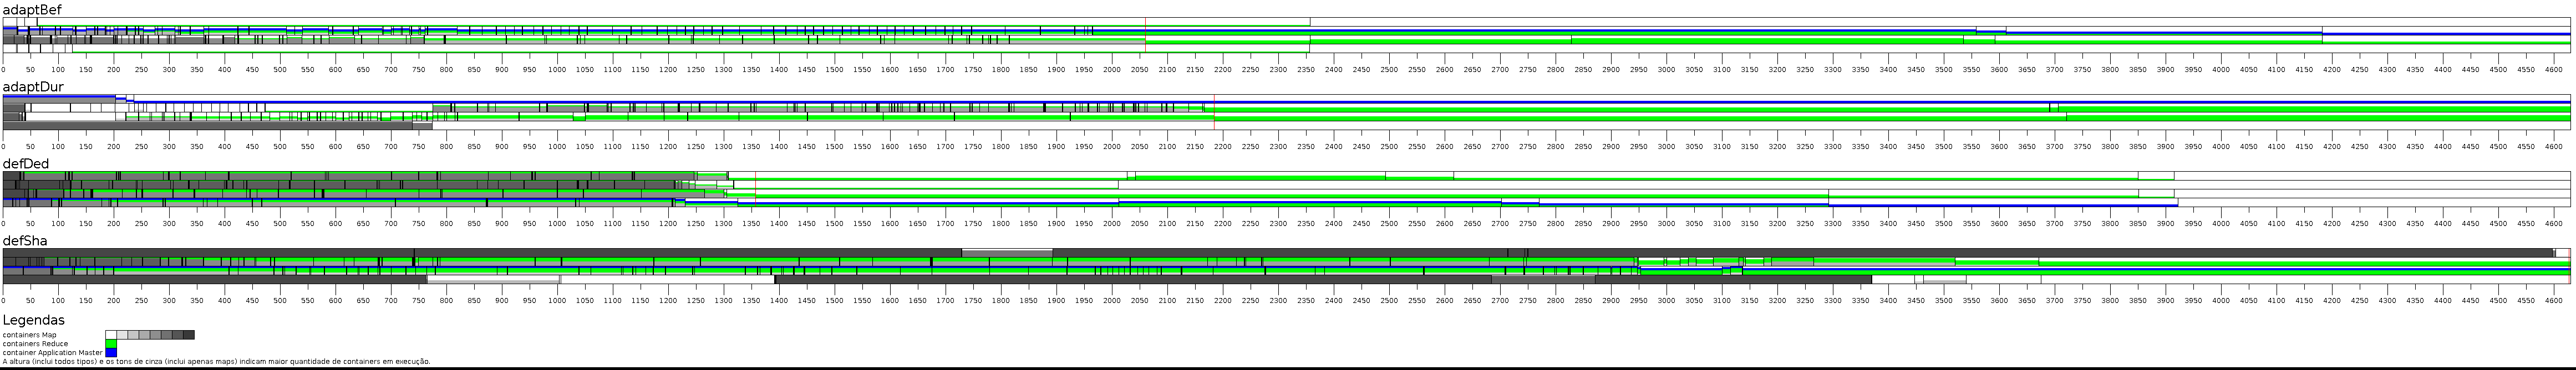
\includegraphics[width=1\textwidth]{figuras/TS-esc-ent.png}
    \caption{Diagrama de Gantt para o experimento em escala (tamanho da entrada) com TeraSort}
	\label{fig:exp3TS}

	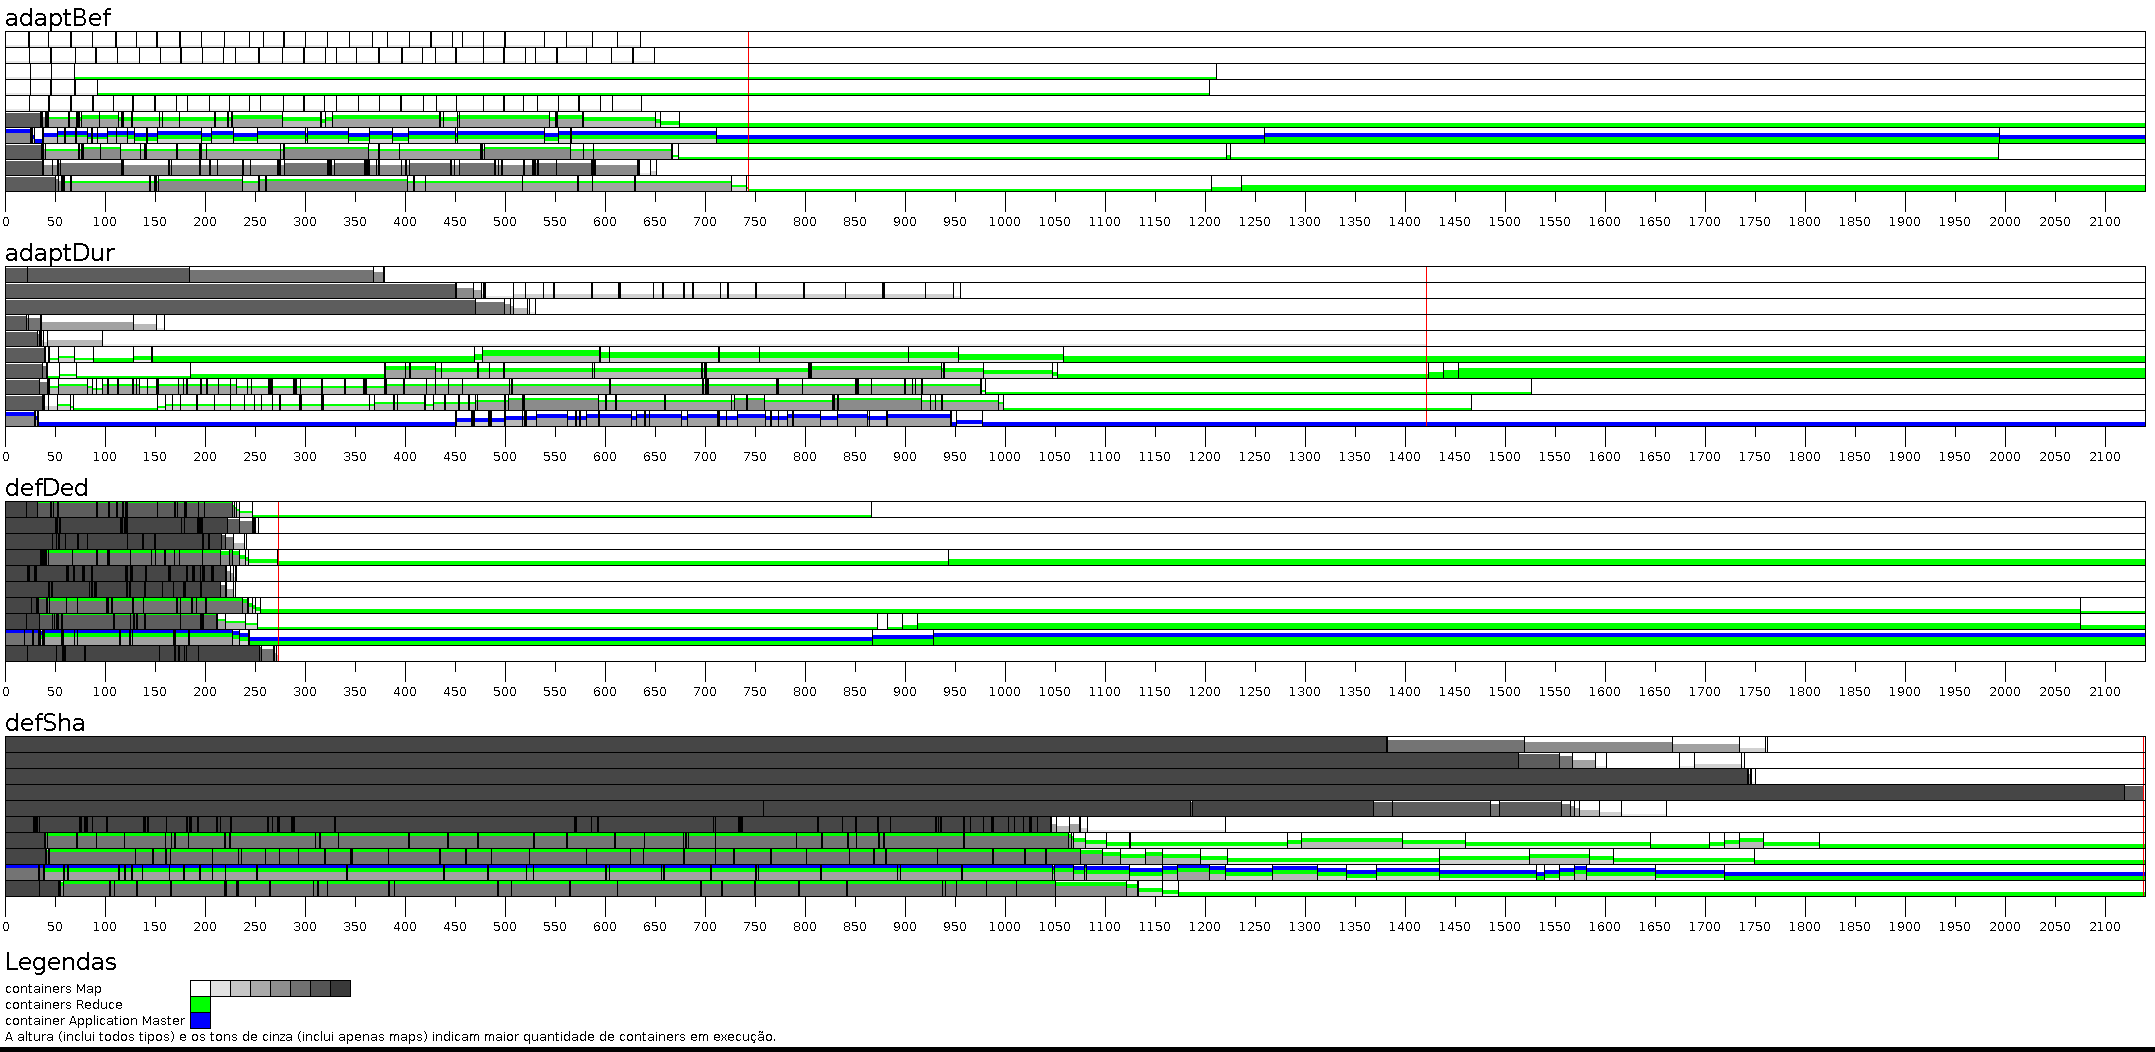
\includegraphics[width=1\textwidth]{figuras/TS-esc-amb.png}
    \caption{Diagrama de Gantt para o experimento em escala (tamanho do ambiente) com TeraSort}
	\label{fig:exp31TS}	
\end{sidewaysfigure}

No experimento realizado com o tamanho da entrada maior pode-se notar que o caso AdaptBef apresentou um tempo de execução mais rápido que o esperado. O tempo de execução atingido foi aproximadamente 50\% maior comparado com o caso DefDed, porém o esperado era de 100\%. Este valor era esperado pois no caso AdaptBef a configuração dos recursos alocáveis é de 2 escravos com 1Gb/core e 2 escravos com 7Gb/cores enquanto a configuração dos recursos alocáveis no caso DefDed é de 4 escravos com 8Gb/cores. Este resultado sugere que desconsiderar os recursos utilizados pelo sistema operacional e serviços do Hadoop já cria uma sobrecarga no nó, porém esta só é perceptível em aplicações que possuem um tempo de execução mais elevado. 

Nota-se, mais uma vez, que os tempos de execução das aplicações apresenta a ordem DefDed, AdaptBef, AdaptDur e DefSha. Contudo, neste experimento a diferença de tempo entre os casos DefSha e AdaptBef, tanto do tempo total como do tempo médio dos \textit{containers} é maior, sugerindo que a solução deste trabalho possui uma efetividade diretamente proporcional ao tamanho da aplicação que é executada. Ainda, o número de tarefas especulativas nos casos DefSha foi muito maior se comparado com os casos onde a solução deste estudo foi implementada.

Os diagramas de Gantt dos experimentos em escala possibilitaram a identificação de outra característica relacionada ao escalonamento, porém esta é uma falha na solução deste estudo. No caso AdaptDur, tanto na escala de entrada como de tamanho do ambiente, é possível identificar zonas onde os nós não sobrecarregados possuem poucos (0-4) \textit{containers}. Este comportamento é causado por uma peculiaridade do Capacity Scheduler, o qual relega o lançamento de \textit{containers} para as filas. Antes da decisão de lançar o \textit{container} ou não, existe um teste que, ao contrário do inicialmente esperado, testa se o total de recursos utilizados \textbf{do \textit{cluster}} é menor que o total de recursos informados. Uma vez que o teste ignora a situação dos recursos específicos de cada nó e é feito com a situação dos recursos do \textit{cluster}, a atualização da capacidade de alguns nós fará com que os recursos utilizados sejam maiores que a capacidade total do \textit{cluster}.

O processo de lançamento sofre influência do recurso de cada nó informado ao escalonador, porém a influência da atualização dos recursos não é local, no sentido de afetar somente o lançamento de \textit{containers} do próprio nó que foi atualizado, mas sim global. Isso implica que a atualização dos recursos de 1 nó infuenciará em todos os \textit{containers} que serão lançados, independentemente de serem lançado ou não no nó que teve seus recursos atualizados. Por exemplo, todos os nós terão inicialmente 7 Gbs de memória e 7 \textit{cores} disponíveis, fazendo com que o \textit{cluster} tenha um total de 70 Gbs e 70 cores. Assim, serão alocados 70 \textit{containers} de 1 Gb de memória e 1 \textit{core} cada. Após o término da alocação, 5 destes nós sofrem atualização dos recursos informados ao escalonador, deixando o \textit{cluster} com um total de 55 Gb e 55 \textit{cores}. Porém, existem 70 \textit{containers} em execução, o que significa que a quantidade de recursos utilizados é de  70 Gb e 70 \textit{cores}. Mesmo que cada um dos 5 nós não sobrecarregados utilizem apenas 2 Gb e 2 \textit{cores} (dos seus 7 disponíveis), caso os \textit{containers} alocados aos nós sobrecarregados não terminem, a utilização do \textit{cluster} continuará acima de 100\% (60 Gb e 60 \textit{cores} usados, 55 Gb e 55 \textit{cores} informados), e portanto, nenhum novo \textit{container} será lançado por mais que existam recursos ociosos em alguns nós.

Para seguir o objetivo inicial de não fazer grandes modificações no algoritmo de escalonamento, seria necessário um controle intermediário da quantidade de recursos disponíveis para o Hadoop e a quantidade de recursos atualmente sendo utilizada pelo Hadoop. Fazendo a redução desta informação no escalonador de forma gradual, à medida que os \textit{containers} finalizam seu processamento. Se este controle for implementado, o problema identificado nestes diagramas de Gantt seria eliminado e não haveriam recursos ociosos em nenhum momento. Ainda assim, os casos que utilizam a solução deste estudo apresentaram um desempenho superior quando comparados com o desempenho da distribuição \textit{default} do Hadoop.


HAHAHA


%
%Analisando as tabelas, é possível identificar alguns padrões. Todos experimentos apresentam um comportamento similar com relação ao tempo total dos \textit{containers Map}: DefDed foi o mais rápido, seguido pelos casos AdaptBef, AdaptDur e finalmente DefSha. Ainda, os casos DefDed e AdaptBef possuem os menores tempos médios de \textit{Map} e estes são muito semelhantes não importando a aplicação analizada. Este comportamento é devido à não sobrecarga dos nós, uma vez que o escalonador possuia os dados corretos com relação aos recursos dos nós durante todo experimento.
%Os diagramas de Gantt também apresentam esta informação uma vez que os experimentos DefDed e AdaptBef possuem tons mais claros e alturas menores do que os demais no início da aplicação, o que significa que há menos \textit{containers} em execução. É possível notar também que o caso AdaptBef leva, em geral, o dobro do tempo do caso DefDed para terminar a etapa de Map. Este resultado é esperado, uma vez que neste experimento o caso DefDed possui o dobro de recursos disponíveis se comparado com o caso AdaptBef. 
%
%Outra observação interessante tem relação com a análise das tarefas especulativas iniciadas em cada aplicação. A aplicação TeraSort possui um número reduzido de tarefas iniciadas e este número é similar em todos os casos. Já o TestDFSIO e o WordCount apresentam um alto número de tarefas especulativas nos casos em que o sistema está sobrecarregado em algum momento (DefSha e AdaptDur). Este comportamento pode ser explicado sob a análise dos fatores que determinam o lançamento ou não de uma tarefa especulativa. Sabe-se que uma tarefa especulativa é iniciada com base numa avaliação de progresso da tarefa, onde uma tarefa atrasada em relação às demais está possivelmente apresentando falhas. No caso do TeraSort, onde as tarefas demandam de maneira uniforme os recursos de memória, CPU e E/S, o tempo de execução está menos sujeito à redução de um recurso específico. Enquanto o TestDFSIO e o WordCount, demandam recursos mais específicos e, portanto, são mais sensíveis à sobrecarga destes recursos. Em todas as aplicações, a utilização de sensibilidade ao contexto como meio de melhorar a adaptabilidade no caso AdaptDur ajuda a reduzir o número de tarefas especulativas quando comparado com o caso DefSha que não apresenta nenhuma capacidade de adaptação à estes ambientes.
%
%Com relação ao fluxo de execução, como ilustrado nos diagramas, é possível notar que os casos DefSha e AdaptDur possuem tons mais escuros no início, o que significa que cada nó está com 16 \textit{containers} em execução (o dobro da capacidade real do nó). Ainda, os primeiros \textit{containers} a terminar nos casos DefDed e AdaptBef levam entre 20 e 50 segundos (conforme linha vertical de segmento), enquanto nos casos DefSha (e em menor grau AdaptDur) os primeiros \textit{containers} levam 70 segundos ou mais para terminar, evidenciando a sobrecarga dos nós. As excessões à esta afirmação são os casos DefSha e AdaptDur do TestDFSIO, nos quais os primeiros \textit{containers} a terem o processamento concluído levam aproximadamente 25 segundos para tal. Através de uma análise mais profunda, é possível notar que todos os casos do experimento TestDFSIO possuem ao menos um seguimento próximo à marca dos 25 segundos, o que significa que uma das tarefas deste conjunto de entrada foi processada rapidamente em todos os casos, e não foi afetada pela sobrecarga dos nós nos casos DefSha e AdaptDur.
%
%Embora os casos DefSha e AdaptDur possuam as mesmas condições iniciais (recursos disponíveis de 50\% e recursos informados de 100\%), o caso AdaptDur necessita de menos tempo para concluir o processamento da aplicação em todas as aplicações. O caso AdaptDur possui uma melhora de 20\% a 40\% no tempo de execução quando comparado com o caso DefSha. A razão para este comportamento é a capacidade de adaptação inserida ao Hadoop, a qual permite que os Node Managers coletem a informação correta e à transmitam para o escalonador, que irá reorganizar a distribuição de tarefas à medida que as tarefas em execução são concluídas. Este comportamento é mais fácil de ser observado nos diagramas das aplicações TeraSort e TestDFSIO. É possível notar também que todos o casos AdaptDur possuem alta concentração de containers no início da aplicação mas essa concentração diminui ao longo da execução, enquanto os casos DefSha mantém a alta concentração até os últimos momentos da execução devido à ausencia de adaptabilidade. Embora o escalonador não preempte \textit{containers} em excesso, é possível observar uma melhora de aproximadamente 40\% no TeraSort e 20\% no TestDFSIO e WordCount apenas pela inibição do lançamento de novos \textit{containers} enquanto o nó está sobrecarregado.
%
%HAHAHAH




%\section{Experimento de medição do \textit{Swap}}
%Uma vez que os experimentos anteriores já responderam algumas questões importantes sobre a viabilidade da solução implementada, este experimento foi realizado com objetivo de analisar se as melhorias no escalonamento são mantidas quando o Hadoop é utilizado em um ambiente ou com uma entrada de dados maior. O experimento utiliza a solução descrita no Capítulo \ref{cap:desen}. A situação expressada com este experimento é de quando os nós do \textit{cluster} começam a ser utilizados por outros usuários antes/durante a aplicação \textit{MapReduce}.

%\subsection{Procedimentos}
%Neste experimento buscou-se analisar o comportamento da solução em um ambiente compartilhado de maior escala que nos experimentos anteriores. Foram feitos 2 experimentos distintos, um com escala de aplicação outro com escala de ambiente. Para a escala de aplicação a única diferença das configurações foi o tamanho da entrada, sendo utilizada uma entrada de 30 Gb para o TeraSort. Para a escala de ambiente, utilizou-se um \textit{cluster} com X escravos, sendo que a proporção de recursos reduzidos/livres continuou a mesma. 

%\subsection{Resultados e Interpretações}
%
%\begin{table}[h!]
%	\caption{Resumo dos resultados do TeraSort em escala (tamanho da entrada) em segundos.} \label{tab:exp3TS}
%	\begin{tabular*}{\hsize}{lllll} %{\hsize}{@{\extracolsep{\fill}}lllll@{}}
%		%\toprule
%		\textbf{Caso} & \textbf{DefDed} & \textbf{DefSha} & \textbf{AdaptBef} & \textbf{AdaptDur}\\
%		\hline
%		Tempo Total de Map ({\it{s}}) & 1357 & 4627 & 2060 & 2184 \\
%		Tempo Médio de Map ({\it{s}}) & 43.39 & 299.70 & 45.36 & 65.00 \\
%		%Desvio Padrão & 15.73 & 59.86 & 18.09 & 29.91 \\
%		\# Tarefas Map & 240 & 240 & 240 & 240 \\
%		\# Tarefas Especulativas & 1 & 27 & 0 & 5 \\
%		%\botrule
%	\end{tabular*}
%\end{table}
%
%
%HAHAHA
%
%Analisando as tabelas, é possível identificar alguns padrões. Todos experimentos apresentam um comportamento similar com relação ao tempo total dos \textit{containers Map}: DefDed foi o mais rápido, seguido pelos casos AdaptBef, AdaptDur e finalmente DefSha. Ainda, os casos DefDed e AdaptBef possuem os menores tempos médios de \textit{Map} e estes são muito semelhantes não importando a aplicação analizada. Este comportamento é devido à não sobrecarga dos nós, uma vez que o escalonador possuia os dados corretos com relação aos recursos dos nós durante todo experimento.
%Os diagramas de Gantt também apresentam esta informação uma vez que os experimentos DefDed e AdaptBef possuem tons mais claros e alturas menores do que os demais no início da aplicação, o que significa que há menos \textit{containers} em execução. É possível notar também que o caso AdaptBef leva, em geral, o dobro do tempo do caso DefDed para terminar a etapa de Map. Este resultado é esperado, uma vez que neste experimento o caso DefDed possui o dobro de recursos disponíveis se comparado com o caso AdaptBef. 
%
%Outra observação interessante tem relação com a análise das tarefas especulativas iniciadas em cada aplicação. A aplicação TeraSort possui um número reduzido de tarefas iniciadas e este número é similar em todos os casos. Já o TestDFSIO e o WordCount apresentam um alto número de tarefas especulativas nos casos em que o sistema está sobrecarregado em algum momento (DefSha e AdaptDur). Este comportamento pode ser explicado sob a análise dos fatores que determinam o lançamento ou não de uma tarefa especulativa. Sabe-se que uma tarefa especulativa é iniciada com base numa avaliação de progresso da tarefa, onde uma tarefa atrasada em relação às demais está possivelmente apresentando falhas. No caso do TeraSort, onde as tarefas demandam de maneira uniforme os recursos de memória, CPU e E/S, o tempo de execução está menos sujeito à redução de um recurso específico. Enquanto o TestDFSIO e o WordCount, demandam recursos mais específicos e, portanto, são mais sensíveis à sobrecarga destes recursos. Em todas as aplicações, a utilização de sensibilidade ao contexto como meio de melhorar a adaptabilidade no caso AdaptDur ajuda a reduzir o número de tarefas especulativas quando comparado com o caso DefSha que não apresenta nenhuma capacidade de adaptação à estes ambientes.
%
%Com relação ao fluxo de execução, como ilustrado nos diagramas, é possível notar que os casos DefSha e AdaptDur possuem tons mais escuros no início, o que significa que cada nó está com 16 \textit{containers} em execução (o dobro da capacidade real do nó). Ainda, os primeiros \textit{containers} a terminar nos casos DefDed e AdaptBef levam entre 20 e 50 segundos (conforme linha vertical de segmento), enquanto nos casos DefSha (e em menor grau AdaptDur) os primeiros \textit{containers} levam 70 segundos ou mais para terminar, evidenciando a sobrecarga dos nós. As excessões à esta afirmação são os casos DefSha e AdaptDur do TestDFSIO, nos quais os primeiros \textit{containers} a terem o processamento concluído levam aproximadamente 25 segundos para tal. Através de uma análise mais profunda, é possível notar que todos os casos do experimento TestDFSIO possuem ao menos um seguimento próximo à marca dos 25 segundos, o que significa que uma das tarefas deste conjunto de entrada foi processada rapidamente em todos os casos, e não foi afetada pela sobrecarga dos nós nos casos DefSha e AdaptDur.
%
%Embora os casos DefSha e AdaptDur possuam as mesmas condições iniciais (recursos disponíveis de 50\% e recursos informados de 100\%), o caso AdaptDur necessita de menos tempo para concluir o processamento da aplicação em todas as aplicações. O caso AdaptDur possui uma melhora de 20\% a 40\% no tempo de execução quando comparado com o caso DefSha. A razão para este comportamento é a capacidade de adaptação inserida ao Hadoop, a qual permite que os Node Managers coletem a informação correta e à transmitam para o escalonador, que irá reorganizar a distribuição de tarefas à medida que as tarefas em execução são concluídas. Este comportamento é mais fácil de ser observado nos diagramas das aplicações TeraSort e TestDFSIO. É possível notar também que todos o casos AdaptDur possuem alta concentração de containers no início da aplicação mas essa concentração diminui ao longo da execução, enquanto os casos DefSha mantém a alta concentração até os últimos momentos da execução devido à ausencia de adaptabilidade. Embora o escalonador não preempte \textit{containers} em excesso, é possível observar uma melhora de aproximadamente 40\% no TeraSort e 20\% no TestDFSIO e WordCount apenas pela inibição do lançamento de novos \textit{containers} enquanto o nó está sobrecarregado.
%
%HAHAHAH
\chapter{Conclusão}
%-------------------------------------------------------------------

No contexto atual do processamento distribuído de dados, uma alternativa que sempre deve ser considerada é a utilização do MapReduce e seus \textit{frameworks} de processamento. Sendo o Hadoop o mais conhecido destes, a sua utilização para o processamento de dados de maneira distribuída vem ganhando mais e mais adeptos. Embora existam serviços que disponibilizem um ambiente na nuvem para que o usuário processe seus dados, algumas pequenas empresas podem preferir outra alternativa à passar seus dados para a nuvem. Nestes casos, pode ser mais simples utilizar os recursos ociosos que estão disponíveis dentro da própria empresa.

Ainda que a utilização dos recursos ociosos da própria empresa pareça mais simples, o Hadoop não é capaz de gerenciar recursos compartilhados em um nó do \textit{cluster}. Este estudo teve como objetivo tornar o Hadoop capaz de suportar compartilhamento de recursos através de um escalonamento adaptativo com relação aos recursos disponíveis. A solução realiza esta tarefa através da coleta e transmissão de dados, em conjunto com a utilização do escalonador Capacity Scheduler. Foram realizados experimentos que apresentavam a degradação de recursos, sendo que esta degradação poderia ocorrer tanto antes do início quanto no decorrer da aplicação de MapReduce. Estes dois cenários foram enfatizados por três fatores: (1) são os cenários que ocorrem mais comumente em ambientes compartilhados; (2) a entrada/saída de nós já é suportado, com algumas peculiaridades, pelo Hadoop; e (3) a reintegração de recursos compartilhados já têm suporte com a solução implementada, porém, comparada à degradação de recursos, não possui impacto significativo no desempenho.

A solução deste estudo foi capaz de melhorar o desempenho nos casos testados com utilização compartilhada do \textit{cluster}. Os resultados alcançados neste estudo indicam que a utilização do Hadoop em um \textit{cluster} compartilhado é possível, mesmo quando este for composto por computadores pertencentes à uma pequena rede empresarial que pode, a qualquer momento, ter a utilização concorrente dos recursos em determinados nós. Como resultado do desenvolvimento deste estudo, apresentou-se uma solução, simples e não intrusiva, para a utilização do Hadoop em ambientes compartilhados. Foram utilizados apenas os recursos que inicialmente são considerados pelo Hadoop (memória e \textit{cores})  para tornar o escalonamento adaptável.

O benefício da utilização da solução deste estudo é decorrente da eliminação ou, nos piores casos, minimização da sobrecarga dos nós em virtude do compartilhamento. O simples fato de inibir o lançamento de novos \textit{containers} quando alguns nós do \textit{cluster} estão sobrecarregados apresentou um ganho de desempenho de até 40\% em alguns casos quando comparado com a distribuição \textit{default} do Hadoop. Mesmo que o ganho de desempenho apresentado seja bom, foi identificada uma falha na solução. Sendo assim, é possível que o ganho de desempenho real seja ainda maior.

Utilizando este estudo como ponto de partida, diversos trabalhos futuros são possíveis. Destacando-se, é claro, um melhor controle dos recursos sobrecarregados para que a falha discutida nos experimentos em escala seja solucionada. Além disso, é possível explorar o Application Master com objetivo de compreender e tornar o gerenciamento interno de cada aplicação adaptativo.

\setlength{\baselineskip}{\baselineskip}

%%=============================================================================
%% Referências
%%=============================================================================
%\renewcommand{\bibname}{References}
\bibliographystyle{abnt}
\bibliography{referencias/referencias}

%IMPORTANTE: Se precisar usar alguma seção ou subseção dentro dos apêndices ou
%anexos, utilizar o comando \tocless para não adicionar no Sumário
%Exemplos: 
% \tocless\section{Histórico}
%%=============================================================================
%% Apêndices
%%=============================================================================
%\renewcommand{\appendixname}{Appendix}
\appendix

\chapter{Grafos gerados referentes ao \emph{ResourceManager}}
\label{chap:ApendA}

A seguir encontram-se uma breve explicação e as figuras geradas pelo segundo método empregado na etapa de estudo da arquitetura do \emph{framework}.

A pertinência das figuras é validada por elas descreverem todos os caminhos possíveis que dada interface pode tomar. O fluxo do caso perfeito seria iniciado com o recebimento de um novo \emph{job} pelo \emph{ResourceManager}. Para que o \emph{job} possa ser iniciado alguns pré-requisitos devem ser satisfeitos. É a partir desse ponto que as figuras entram em cena.

Para que uma aplicação seja iniciada, primeiramente é criado um \emph{AppAttempt}. O \emph{AppAttempt} é literalmente uma tentativa de aplicação, pela qual o \emph{ResourceManager} tentará alocar os recursos necessários (\emph{Node e Container}) para que essa aplicação seja realmente criada e submetida ao cluster. Durante o processo do \emph{RMAppAttempt} o \emph{ResourceManager} irá tentar alocar um ou mais \emph{RMContainers} bem como \emph{RMNodes} para que a aplicação tenha recursos suficientes para sua execução. Após os recursos necessários terem sido alocados com sucesso, a aplicação passa para o status de \emph{RMApp} e é submetida ao cluster.

%IMPORTANTE: Se precisar usar alguma seção ou subseção dentro dos apêndices ou
%anexos, utilizar o comando \tocless para não adicionar no Sumário
%Exemplos: 
% \tocless\section{Histórico}
% \tocless\subsection{Detalhes}
%\tocless\section{teste}
%Este é um teste de seção dentro do apêndice

\begin{figure}[hbtn]
   \centering
   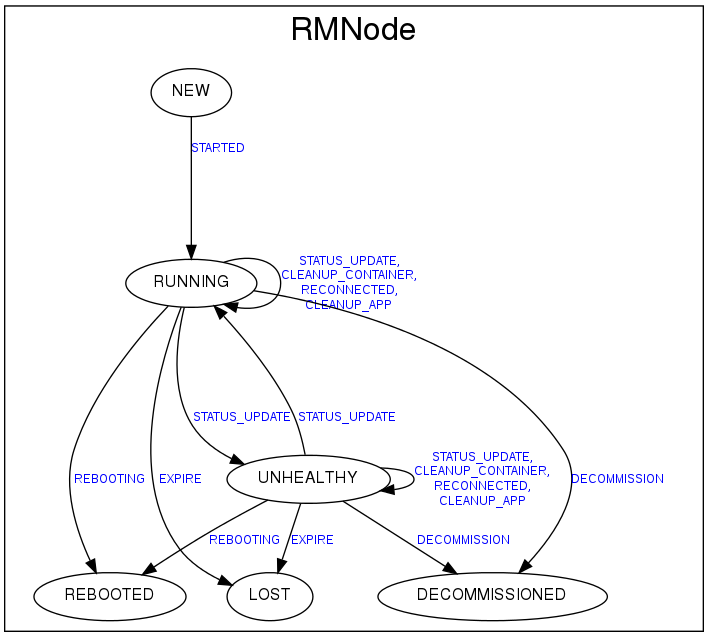
\includegraphics[width=12cm]{figuras/Figura05-RMNode.png}
   \caption{Máquina de estados do RMNode}
   \label{fig:RMNode}
\end{figure}

\begin{figure}[hbtn]
   \centering
   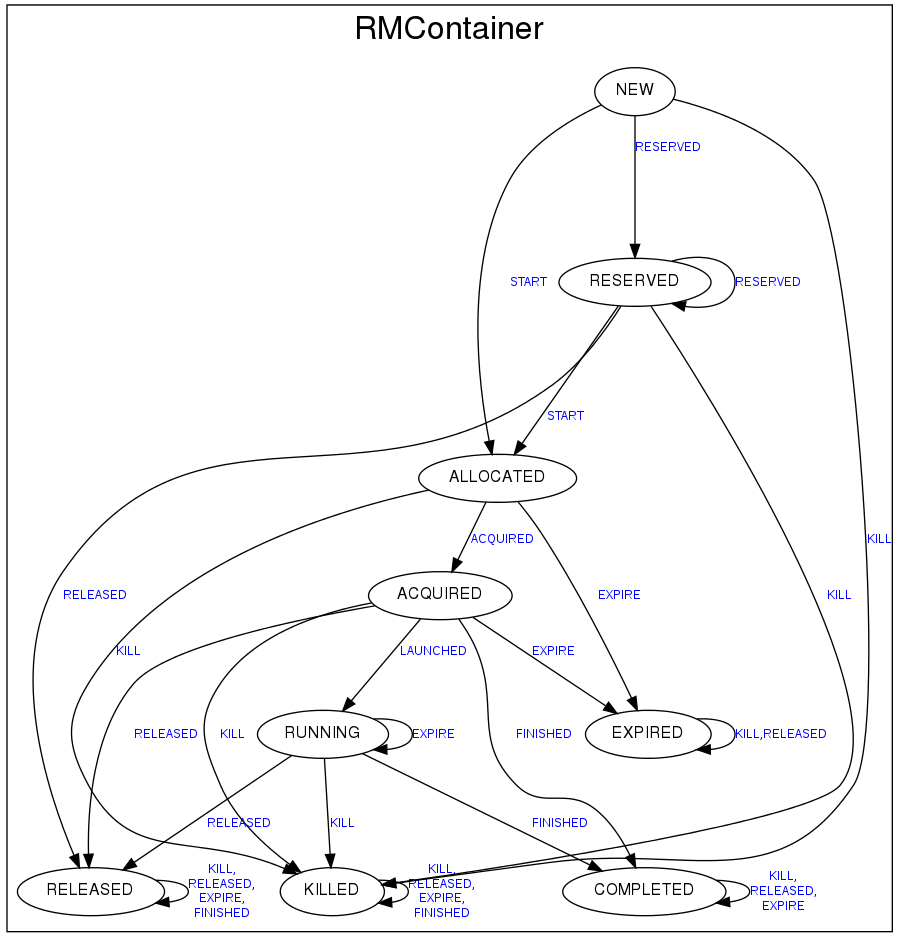
\includegraphics[width=15cm]{figuras/Figura03-RMContainer.png}
   \caption{Máquina de estados do RMContainer}
   \label{fig:RMContainer}
\end{figure}

\begin{figure}[hbtn]
   \centering
   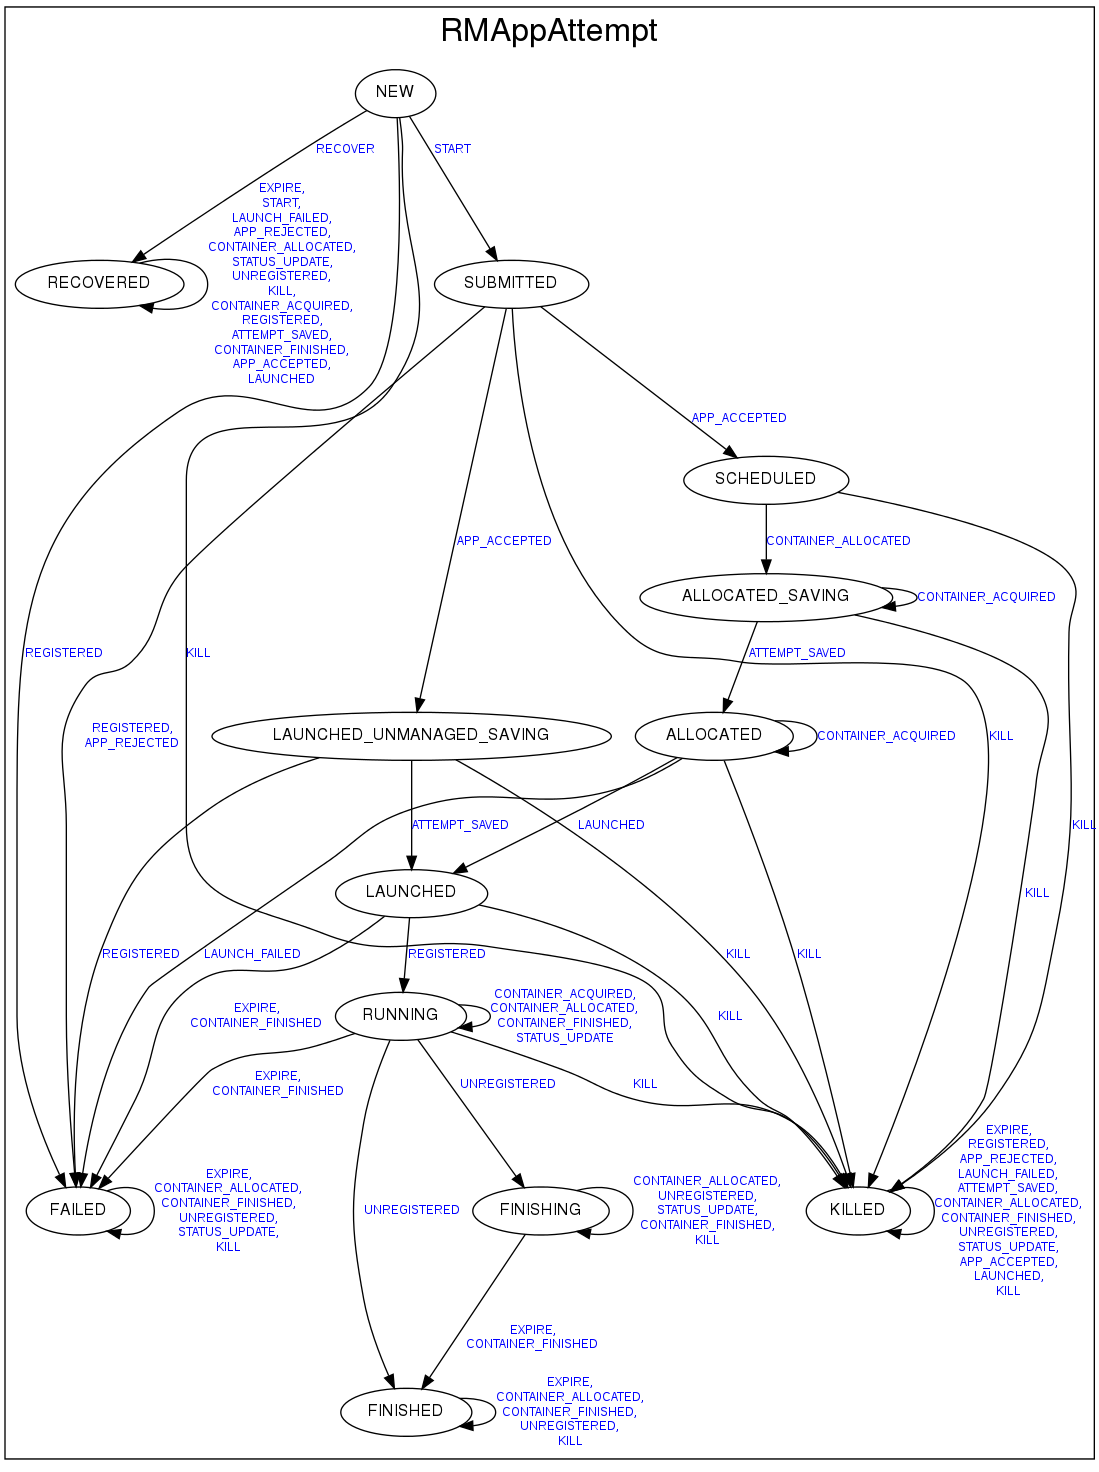
\includegraphics[width=15cm]{figuras/Figura02-RMAppAttempt.png}
   \caption{Máquina de estados do RMAppAttempt}
   \label{fig:RMAppAttempt}
\end{figure}

\begin{figure}[hbtn]
   \centering
   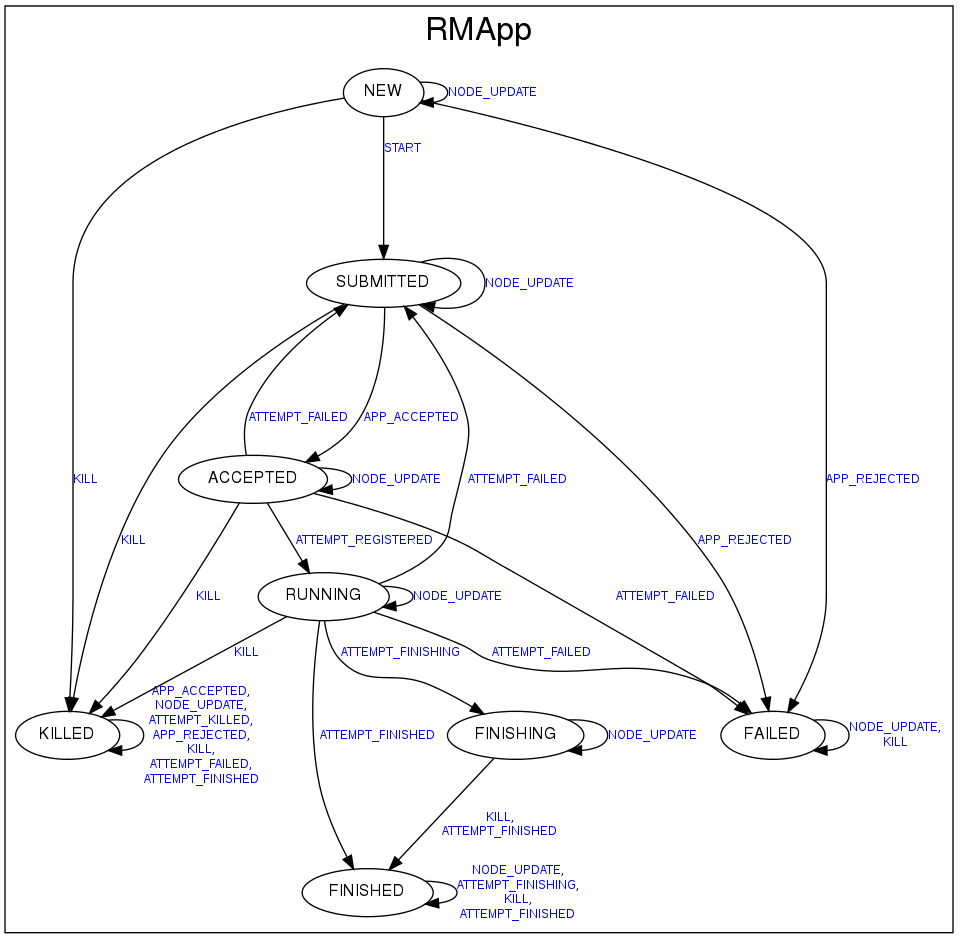
\includegraphics[width=15cm]{figuras/Figura04-RMApp.png}
   \caption{Máquina de estados do RMApp}
   \label{fig:RMApp}
\end{figure}
\chapter{Grid'5000 execution environment configuration}

This appendix has the necessary steps in order to setup a correctly working execution environment on Grid'5000 cluster.

The Apache Hadoop's installation, contrary to end users standard program installations, doesn't have a graphical interface. Actually the installation is just the extraction of files to a determined folder, however the environment configuration isn't trivial and demands some network administration knowledge.

For the correct functioning of the framework, it is necessary to edit of some files responsible for describing the environment in which it will execute. Besides, it is necessary to have a network in which every node has access to the others. Knowing that Apache Hadoop has suffered some heavy changes in changing from 1.x to 2.x, it was expected that installing both versions would make the differences clearer.

In the beginning of this work the objective was to install and configure the Apache Hadoop in three situations:
\begin{itemize}
        \item localhost, a single-node case.
        \item mini cluster, a multi-node case.
        \item Grid'5000, another multi-node case.
\end{itemize}

There are two configuration steps, the network step which refers to the configuration that doesn't depend on Hadoop and the Hadoop step which refers to the parameters that influence Hadoop's execution. This step is composed of tasks executed on the operational system, such as the user creation and ssh configuration. The second step, on the other hand, is the proper Hadoop environment configuration and, therefore, it has to change some configuration files in a way that Hadoop can be executed without errors.

The OS configuration is equal on both versions, since it has already been noted that it is independent of Hadoop. The Hadoop configuration, however, has a few differences between versions. Even so, both versions follow the same general rules. The Hadoop configuration is made through a bunch of xml files already mentioned in section \ref{chap:fundamentacao}, subsection \ref{sec:envconfig}, in which some properties containing name and value are inserted. This properties will be responsible for changing the default Hadoop behavior, but aside some properties changing their names, the biggest difference is that YARN version has a new xml file named \textit{yarn-site.xml}, it contains all parameters related to the YARN framework and therefore has a high influence on MapReduce and job execution performance.

Initially it was chosen to configure both versions on every specified instance, however, given the project focus the version 1.x was no longer a viable alternative and it's use was discontinued.

The localhost environment configuration, is a simple process and occurred  without problems after a basic contact with the framework. The mini cluster environment, was configured using two machines, already presenting a difference, in which the master could also be a slave on 1.x, in other words, it was possible to run NameNode and DataNode on the same node. On YARN version, the NameNode machine can't start a DataNode service, and the same is valid for ResourceManager and NodeManager. This change makes the tasks of processing and management totally apart and differentiable making the cluster more organized.

The real experiment starts when the Hadoop is deployed on a real cluster, like the Grid'5000, it was decided to use only the YARN version from this point onward. The installation of YARN requires only a few changes from mini cluster to Grid'5000 environment. The Grid also supplies a lot of tools that makes the job easier for Hadoop management.

At the end of this stage, some Hadoop peculiarities have already been cleared and the execution environment for posterior testing of the implementations was already deployed. Also, it is important to note that it was possible to identify some contexts that would present a high difficult to change the behavior. One of these behaviors would be the addition or removal of nodes on real time after the cluster initialization. The difficult comes from the way the service uses static reference to xml files that are read only on the initialization, making it impossible to use their values without restarting the services.

\chapter{Source code edition and compilation}
This appendix has the necessary steps in order to setup a correctly working compilation environment.

Given the project nature of generating a improved, context-aware, scheduler for the Apache Hadoop, it is necessary that this scheduler is included on the final distribution. Not only it has to be included, it has to be available for use by everyone who wants to try it. In order to achieve this, new jar files have to be generated from the modified code. Because of this a previous study was made about the necessary requisites in order to compile and generate these jar files.

The study began with the official documentation consultation, which included Apache Hadoop web site and help files included on the source code distributions. This way it was possible to create some steps required to compile the code. Starting from this list it was possible to identify the required dependencies to compile the code, which were then installed. The dependencies were: JDK 1.6 or higher, Maven 3.0, ProtocolBuffer 2.4.1 or higher and Cmake2.6 or higher.

The greatest objective of this process was to discover how the compilation took place and also how it would behave with the addition of new classes to standard code. Aiming to achieve this objective, a new but simple scheduler class was added. After the compilation process ended, the generated jar files were then copied to the Grid'5000 and deployed there in order to test if it would be possible to execute the compiled version in that environment.

Once the Hadoop services were deployed, it could be proven that the new scheduler was being used. It was also possible to identify the same vulnerability in the previous stage, in which the service has to be restarted in order to modify some of the Hadoop's parameters. 
\chapter{Example of semi-processed log from a experiment}
\label{chap:logs}

The experiment results were collected using the Log System from Hadoop. Here is an example of a log already semi-processed, which means that this log has been filtered to show only the entries relevant to the analysis.

The following log snippet, shows the log when an application was submitted, in this case the application was the TeraSort. It is possible to note a lot of information, like the user who submitted and queue used, the applicationId, among others.

\lstset{language=Java,
             basicstyle=\footnotesize,
             numbers=left,
             extendedchars=\true
             showspaces = false,
             numberstyle=\footnotesize,
             frame=shadowbox,
             breaklines = true}

\begin{lstlisting}
2014-01-13 13:19:21,517 INFO org.apache.hadoop.yarn.server.resourcemanager.scheduler.capacity.LeafQueue: Application application_1389615375211_0002 from user: hadoop activated in queue: default
2014-01-13 13:19:21,518 INFO org.apache.hadoop.yarn.server.resourcemanager.scheduler.capacity.LeafQueue: Application added - appId: application_1389615375211_0002 user: org.apache.hadoop.yarn.server.resourcemanager.scheduler.capacity.LeafQueue$User@5673e296, leaf-queue: default #user-pending-applications: 0 #user-active-applications: 1 #queue-pending-applications: 0 #queue-active-applications: 1
\end{lstlisting}

Another interesting log snippet is the one that show the assignment and completion of containers. The following snippet shows when the Reduce and ApplicationMaster containers are completed and the application is finished.

\begin{lstlisting}
2014-01-13 13:24:05,016 INFO org.apache.hadoop.yarn.server.resourcemanager.scheduler.capacity.LeafQueue: completedContainer container=Container: [ContainerId: container_1389615375211_0002_01_000040, NodeId: stremi-44.reims.grid5000.fr:34048, NodeHttpAddress: stremi-44.reims.grid5000.fr:8042, Resource: <memory:4830, vCores:1>, Priority: 10, Token: Token { kind: ContainerToken, service: 172.16.160.44:34048 }, ] resource=<memory:4830, vCores:1> queue=default: capacity=1.0, absoluteCapacity=1.0, usedResources=<memory:4830, vCores:1>usedCapacity=0.024998447, absoluteUsedCapacity=0.024998447, numApps=1, numContainers=1 usedCapacity=0.024998447 absoluteUsedCapacity=0.024998447 used=<memory:4830, vCores:1> cluster=<memory:193212, vCores:96>
2014-01-13 13:24:11,146 INFO org.apache.hadoop.yarn.server.resourcemanager.scheduler.capacity.LeafQueue: default used=<memory:0, vCores:0> numContainers=0 user=hadoop user-resources=<memory:0, vCores:0>
2014-01-13 13:24:11,147 INFO org.apache.hadoop.yarn.server.resourcemanager.scheduler.capacity.LeafQueue: completedContainer container=Container: [ContainerId: container_1389615375211_0002_01_000001, NodeId: stremi-7.reims.grid5000.fr:58215, NodeHttpAddress: stremi-7.reims.grid5000.fr:8042, Resource: <memory:4830, vCores:1>, Priority: 0, Token: Token { kind: ContainerToken, service: 172.16.160.7:58215 }, ] resource=<memory:4830, vCores:1> queue=default: capacity=1.0, absoluteCapacity=1.0, usedResources=<memory:0, vCores:0>usedCapacity=0.0, absoluteUsedCapacity=0.0, numApps=1, numContainers=0 usedCapacity=0.0 absoluteUsedCapacity=0.0 used=<memory:0, vCores:0> cluster=<memory:193212, vCores:96>
2014-01-13 13:24:11,150 INFO org.apache.hadoop.yarn.server.resourcemanager.scheduler.capacity.LeafQueue: Application removed - appId: application_1389615375211_0002 user: hadoop queue: default #user-pending-applications: 0 #user-active-applications: 0 #queue-pending-applications: 0 #queue-active-applications: 0
\end{lstlisting}

Finally, there is something that influences a lot on the results, which is the time that an action took place. As it was possible to see on the above examples, the Hadoop Log System provides the hour, minute, second and milliseconds information. Thanks to this, two assignments that happened with mere milliseconds of difference were shown as 1 second delayed on chapter \ref{chap:Experiments and Results}. The first container belongs to node stremi-44 and started at 13:19:29,995. The second container belongs to stremi-42 and started at 13:19:30:079

\begin{lstlisting}
2014-01-13 13:19:29,995 INFO org.apache.hadoop.yarn.server.resourcemanager.scheduler.capacity.LeafQueue: assignedContainer application=application_1389615375211_0002 container=Container: [ContainerId: container_1389615375211_0002_01_000030, NodeId: stremi-44.reims.grid5000.fr:34048, NodeHttpAddress: stremi-44.reims.grid5000.fr:8042, Resource: <memory:4830, vCores:1>, Priority: 20, Token: Token { kind: ContainerToken, service: 172.16.160.44:34048 }, ] containerId=container_1389615375211_0002_01_000030 queue=default: capacity=1.0, absoluteCapacity=1.0, usedResources=<memory:140070, vCores:29>usedCapacity=0.72495496, absoluteUsedCapacity=0.72495496, numApps=1, numContainers=29 usedCapacity=0.72495496 absoluteUsedCapacity=0.72495496 used=<memory:140070, vCores:29> cluster=<memory:193212, vCores:96>
2014-01-13 13:19:30,079 INFO org.apache.hadoop.yarn.server.resourcemanager.scheduler.capacity.LeafQueue: assignedContainer application=application_1389615375211_0002 container=Container: [ContainerId: container_1389615375211_0002_01_000031, NodeId: stremi-42.reims.grid5000.fr:43999, NodeHttpAddress: stremi-42.reims.grid5000.fr:8042, Resource: <memory:4830, vCores:1>, Priority: 20, Token: Token { kind: ContainerToken, service: 172.16.160.42:43999 }, ] containerId=container_1389615375211_0002_01_000031 queue=default: capacity=1.0, absoluteCapacity=1.0, usedResources=<memory:144900, vCores:30>usedCapacity=0.74995345, absoluteUsedCapacity=0.74995345, numApps=1, numContainers=30 usedCapacity=0.74995345 absoluteUsedCapacity=0.74995345 used=<memory:144900, vCores:30> cluster=<memory:193212, vCores:96>
\end{lstlisting}

\chapter{Main code changes performed}
\label{chap:codechanges}

The changes that had the greatest impact on the behavior were the collector integration and the allocation re-scaling. The collector code is available on the link at the references, therefore, only the usage of the package will be inserted here in comparison to the original.

\lstset{language=Java,
             basicstyle=\footnotesize,
             numbers=left,
             extendedchars=\true
             showspaces = false,
             numberstyle=\footnotesize,
             frame=shadowbox,
             breaklines = true}

Starting with the original NodeManager creation, in which the totalResources are gotten. Note how the memoryMB and virtualCores variables are taken from the conf, which is the pointer to the default xml file. This method is from the NodeStatusUpdaterImpl class.

\begin{lstlisting}

protected void serviceInit(Configuration conf) throws Exception {
    int memoryMb = 
        conf.getInt(
            YarnConfiguration.NM_PMEM_MB, YarnConfiguration.DEFAULT_NM_PMEM_MB);
    float vMemToPMem =             
        conf.getFloat(
            YarnConfiguration.NM_VMEM_PMEM_RATIO, 
            YarnConfiguration.DEFAULT_NM_VMEM_PMEM_RATIO); 
    int virtualMemoryMb = (int)Math.ceil(memoryMb * vMemToPMem);
    
    int virtualCores =
        conf.getInt(
            YarnConfiguration.NM_VCORES, YarnConfiguration.DEFAULT_NM_VCORES);

    this.totalResource = recordFactory.newRecordInstance(Resource.class);

    this.totalResource.setMemory(memoryMb);
    this.totalResource.setVirtualCores(virtualCores);
	metrics.addResource(totalResource);
    this.tokenKeepAliveEnabled = isTokenKeepAliveEnabled(conf);
    this.tokenRemovalDelayMs =
        conf.getInt(YarnConfiguration.RM_NM_EXPIRY_INTERVAL_MS,
            YarnConfiguration.DEFAULT_RM_NM_EXPIRY_INTERVAL_MS);
    
    // Default duration to track stopped containers on nodemanager is 10Min.
    // This should not be assigned very large value as it will remember all the
    // containers stopped during that time.
    durationToTrackStoppedContainers =
        conf.getLong(YARN_NODEMANAGER_DURATION_TO_TRACK_STOPPED_CONTAINERS,
          600000);
    if (durationToTrackStoppedContainers < 0) {
      String message = "Invalid configuration for "
        + YARN_NODEMANAGER_DURATION_TO_TRACK_STOPPED_CONTAINERS + " default "
          + "value is 10Min(600000).";
      LOG.error(message);
      throw new YarnException(message);
    }
    if (LOG.isDebugEnabled()) {
      LOG.debug(YARN_NODEMANAGER_DURATION_TO_TRACK_STOPPED_CONTAINERS + " :"
        + durationToTrackStoppedContainers);
    }
    super.serviceInit(conf);
    LOG.info("Initialized nodemanager for " + nodeId + ":" +
        " physical-memory=" + memoryMb + " virtual-memory=" + virtualMemoryMb +
        " virtual-cores=" + virtualCores);
  }
\end{lstlisting}

Then the changes made in the method to enable collectors. The rest of the method was not altered. The reason for the double casting is that the collector returns a Float and Double value and it's not possible to cast directly to int.

\begin{lstlisting}
protected void serviceInit(Configuration conf) throws Exception {
	PhysicalMemoryCollector memoryCollector = new PhysicalMemoryCollector();
    TotalProcessorsCollector processorsCollector = new TotalProcessorsCollector();

    int memoryMb = (int)(float)memoryCollector.collect().get(0)/1024;
    int virtualCores = (int)(double)processorsCollector.collect().get(0);

    this.totalResource = recordFactory.newRecordInstance(Resource.class);
\end{lstlisting}

The other change that had a strong impact in CapacityScheduler behavior was the insertion of recalculations of allocation limits inside the addNode method. This method belongs to the CapacityScheduler class. Starting with the original code.

\begin{lstlisting}
private synchronized void addNode(RMNode nodeManager) {
    this.nodes.put(nodeManager.getNodeID(), new FiCaSchedulerNode(nodeManager,
        usePortForNodeName));
    Resources.addTo(clusterResource, nodeManager.getTotalCapability());
    root.updateClusterResource(clusterResource);
    ++numNodeManagers;
  }
\end{lstlisting}

The same changes made on the addNode were also made on removeNode. Thus, when a node is killed, or is not accessible for a long period, it will be removed and the limits will be adjusted too.

\begin{lstlisting}
private synchronized void addNode(RMNode nodeManager) {
    this.nodes.put(nodeManager.getNodeID(), new FiCaSchedulerNode(nodeManager,
        usePortForNodeName));
    Resource oldCap = Resources.clone(clusterResource);
    Resources.addTo(clusterResource, nodeManager.getTotalCapability());
    root.updateClusterResource(clusterResource);
    ++numNodeManagers;
    LOG.info("MEU Added node " + nodeManager.getNodeAddress() +
        " clusterResource before: " + oldCap + " nodecapability: " + nodeManager.getTotalCapability() + " clusterResource now: " + clusterResource);
    LOG.info("MEU Changing allocation minimum & maximum. Actual minimum: " + this.minimumAllocation + "actual maximum: " + this.maximumAllocation + ".\nDefault settings: cluster must have capacity for at least " + minimumContainers + " containers, and no more than " + maximumContainers + "containers. 8GB RAM cluster would have 1GB minimum/maximum, 80GB RAM cluster would have 4GB minimum and 10GB maximum.");
    this.minimumAllocation.setMemory(clusterResource.getMemory() / maximumContainers);
    this.minimumAllocation.setVirtualCores(clusterResource.getVirtualCores() / maximumContainers);
    this.maximumAllocation.setMemory(clusterResource.getMemory() / minimumContainers);
    this.maximumAllocation.setVirtualCores(clusterResource.getVirtualCores() / minimumContainers);
    if (this.minimumAllocation.getMemory() < minimumMemory)
       this.minimumAllocation.setMemory(minimumMemory);
    if (this.minimumAllocation.getVirtualCores() < minimumVcores)
       this.minimumAllocation.setVirtualCores(minimumVcores);
    if (this.maximumAllocation.getMemory() < this.minimumAllocation.getMemory())
       this.maximumAllocation = this.minimumAllocation;
    LOG.info("MEU New minimumAllocation settings: " + minimumAllocation + "\nNew maximumAllocation settings: " + maximumAllocation);
\end{lstlisting}

%%=============================================================================
%% Anexos
%%=============================================================================
%\annex
%
\chapter{Questionários aplicados para a Análise de Tarefas}



%
\chapter{Resultados da Análise de Casos de Uso}
\begin{figure}[hbtn]
   \centering
   \includegraphics[width=6.5cm]{figuras/figura09-anexob.eps}
   \caption{Análise dos pincipais Portais da área de Informática de instituições federias}
   \label{fig:CASOSDEUSO}
\end{figure}

\end{document}
